\documentclass[11pt, a4paper, notitlepage]{report}

\usepackage{amsmath, amssymb, amsthm}
\usepackage{geometry}
\geometry{margin=1in}
\usepackage{microtype}           % microtypography: prevents most overfull hboxes
\usepackage{hyperref}
\hypersetup{colorlinks=true, linkcolor=blue!60!black, urlcolor=blue!60!black,
            breaklinks=true}     % allow URLs to break across lines
\usepackage{xurl}                % aggressive URL line-breaking (load AFTER hyperref)
\usepackage{enumitem}
\usepackage{algorithm}
\usepackage{algpseudocode}
\usepackage{listings}
\usepackage{xcolor}
\usepackage[most]{tcolorbox}
\tcbuselibrary{theorems}
\usepackage{titlesec}
\usepackage{booktabs}
\usepackage{array}
\usepackage{tabularx}           % auto-width columns that wrap text
\usepackage{tikz}
\usetikzlibrary{arrows.meta, shapes.geometric, positioning, fit, calc, matrix, decorations.pathreplacing}
\setcounter{secnumdepth}{3}

% ── Overflow prevention ───────────────────────────────────────────────────────
\sloppy
\setlength{\emergencystretch}{3em}

% ── Highlight boxes ───────────────────────────────────────────────────────────
\newtcolorbox{keyresult}[1][]{
  enhanced, colback=blue!5!white, colframe=blue!60!black,
  fonttitle=\bfseries, title={Key Result}, #1
}
\newtcolorbox{examtip}[1][]{
  enhanced, colback=green!5!white, colframe=green!50!black,
  fonttitle=\bfseries, title={Exam Tip}, #1
}
\newtcolorbox{warning}[1][]{
  enhanced, colback=red!5!white, colframe=red!60!black,
  fonttitle=\bfseries, title={Warning}, #1
}

% ── Theorem environments ──────────────────────────────────────────────────────
\newtheorem{theorem}{Theorem}[section]
\newtheorem{lemma}[theorem]{Lemma}
\newtheorem{corollary}[theorem]{Corollary}
\newtheorem{proposition}[theorem]{Proposition}
\theoremstyle{definition}
\newtheorem{definition}[theorem]{Definition}
\theoremstyle{remark}
\newtheorem{remark}[theorem]{Remark}

% ── Example environment (amsthm) ─────────────────────────────────────────────
% Plain amsthm theorem style. Usage:
%   \begin{example}[Title]   -> "Example 1.3 (Title)"
%   \begin{example}          -> "Example 1.4"
%   \label{ex:...} / \ref{ex:...} for cross-references (place \label inside)
\theoremstyle{definition}
\newtheorem{example}[theorem]{Example}

% ── Code listings ─────────────────────────────────────────────────────────────
\definecolor{codebg}{RGB}{245,247,250}
\definecolor{codeborder}{RGB}{180,190,210}
\definecolor{codekw}{RGB}{0,80,180}
\definecolor{codecomment}{RGB}{100,110,130}
\definecolor{codestring}{RGB}{160,40,40}

\lstset{
  basicstyle=\ttfamily\footnotesize,
  keywordstyle=\color{codekw}\bfseries,
  commentstyle=\color{codecomment}\itshape,
  stringstyle=\color{codestring},
  breaklines=true,
  breakatwhitespace=false,
  breakautoindent=true,
  postbreak=\mbox{\textcolor{codecomment}{$\hookrightarrow$}\space},
  columns=flexible,
  backgroundcolor=\color{codebg},
  frame=single,
  frameround=ffff,
  framesep=5pt,
  rulecolor=\color{codeborder},
  aboveskip=6pt,
  belowskip=6pt,
  xleftmargin=6pt,
  xrightmargin=6pt,
  numbers=left,
  numberstyle=\ttfamily\tiny\color{codecomment},
  numbersep=8pt,
  showstringspaces=false,
  tabsize=4
}

% ── Suppress forced page break in \tableofcontents ────────────────────────────
\makeatletter
\renewcommand\tableofcontents{%
  \section*{\contentsname}%
  \@starttoc{toc}%
}
\makeatother

% ── Chapter title formatting ──────────────────────────────────────────────────
\titleformat{\chapter}[display]
  {\normalfont\LARGE\bfseries}
  {\chaptertitlename\ \thechapter}{12pt}{\Huge}
\titlespacing*{\chapter}{0pt}{20pt}{30pt}

% ── Title block (filled in by generation script) ──────────────────────────────
% \title{\textbf{<Course Code>: <Course Name>}\\[0.5em]
%        \large <Subtitle>}
% \author{}
% \date{}

\title{\textbf{SC1006: Computer Organisation and Architecture}\\[0.5em]
       \large Weeks 8--9 — Signal Chain, Data Transfer \& Memory Sub-Systems}
\author{}
\date{}

\begin{document}
\maketitle
\tableofcontents

\setcounter{chapter}{8}

% ════════════════════════════════════════════════════════════════════════════
\chapter{Signal Chain \& Data Transfer Sub-Systems}
\label{ch:week9-signal}
% ════════════════════════════════════════════════════════════════════════════

% ════════════════════════════════════════════════════════════════════════════
\section{Signal Chain Sub-System}
\label{ch:signal-chain}
% ════════════════════════════════════════════════════════════════════════════

\subsection{Overview of Computer Sub-Systems}
\label{sec:subsystems-overview}

A modern computer is most naturally understood by decomposing it into a set of cooperating sub-systems. The three principal groups covered in the second half of SC1006 are:

\begin{itemize}
  \item \textbf{Signal Chain Sub-System} — ADC/DAC conversion, parallel and serial digital interfaces, the Direct Memory Access (DMA) controller, and the Interrupt Controller.
  \item \textbf{Memory Sub-System} — SRAM, DRAM, Flash, SSDs, HDDs, Cache, and Virtual Memory.
  \item \textbf{Communication and User Interface Sub-System} — Wired (USB, SATA, HDMI), Wireless (Wi-Fi, Bluetooth), input and output peripherals.
\end{itemize}

This chapter focuses on the signal chain, which bridges the real world (inherently analog) and the digital processor.

\subsection{Signals: Analog and Digital}
\label{sec:signals}

\begin{definition}[Signal]
  \label{def:signal}
  A \emph{signal} is any real-valued function that varies in time and/or space. Examples include audio waveforms, electrocardiograms (ECG), and pulse trains.
\end{definition}

All real-world physical quantities—sound, light, heat, pressure—are \emph{analog}: their magnitude varies continuously both in value and in time. Historically, processing was carried out entirely in the analog domain (e.g., analog equalizers, TV brightness control). Over the past 40 years, digital processors have become sufficiently economical and flexible to displace analog circuitry as the dominant processing platform, primarily because digital representations are highly tolerant of noise and component aging.

\subsection{Analog-to-Digital and Digital-to-Analog Conversion}
\label{sec:adc-dac}

Since a digital processor operates exclusively on discrete binary values, any analog real-world signal must be \emph{digitized} before processing and \emph{reconstructed} afterward.

\subsubsection{Sampling and Quantization}

The analog signal is sampled at discrete time intervals called the \emph{sampling interval} $T_s$. At each sampling point the instantaneous signal level is mapped to the nearest discrete voltage level permitted by the digitization process. For an $n$-bit ADC there are $2^n$ discrete output levels (e.g., a 3-bit ADC has levels $000_2$ through $111_2$, i.e.\ 8 levels).

\begin{keyresult}[title={Key Result: Nyquist Sampling Theorem}]
  The sampling frequency $f_s$ must satisfy
  \[
    f_s \geq 2\,f_{\max},
  \]
  where $f_{\max}$ is the highest frequency component present in the analog signal. Sampling below this rate causes \emph{aliasing} — the reconstructed signal will be incorrect.
\end{keyresult}

\subsubsection{Digital-to-Analog Reconstruction}

After digital processing, the DAC converts the discrete output sequence back to an analog signal. A \emph{smoothing (low-pass) filter} is applied post-DAC to interpolate between the discrete output steps and recover a continuous waveform.

\subsection{Electrical Signal Interfaces}
\label{sec:electrical-interface}

\begin{definition}[Interface]
  \label{def:interface}
  An \emph{interface} is the boundary at which two or more devices meet to exchange information. Data may be transferred serially (one bit at a time on a single line) or in parallel (multiple bits simultaneously on a bus), and each mode may be unidirectional or bidirectional.
\end{definition}

For two devices to communicate correctly, two conditions must be satisfied simultaneously:
\begin{enumerate}
  \item \textbf{Electrical signal level compatibility} — the voltage levels used by each device must be mutually recognizable.
  \item \textbf{Communication protocol compatibility} — both devices must speak the same handshaking and data protocol.
\end{enumerate}

\subsubsection{Logic Level Parameters}
\label{sec:logic-levels}

Digital data is encoded as logic \texttt{0} or \texttt{1} via voltage levels. Four device parameters define whether two devices can communicate:

\begin{center}
\renewcommand{\arraystretch}{1.3}
\begin{tabular}{>{\ttfamily}cl}
  \toprule
  \normalfont Parameter & Definition \\
  \midrule
  VOH & Minimum output voltage guaranteed for a transmitted logic \texttt{1} \\
  VOL & Maximum output voltage guaranteed for a transmitted logic \texttt{0} \\
  VIH & Minimum input voltage that the receiver recognizes as logic \texttt{1} \\
  VIL & Maximum input voltage that the receiver recognizes as logic \texttt{0} \\
  \bottomrule
\end{tabular}
\end{center}

\begin{keyresult}[title={Key Result: Logic Level Compatibility Conditions}]
  For device A (transmitter) and device B (receiver) to communicate without error:
  \[
    \mathrm{VOH}_A \geq \mathrm{VIH}_B \qquad \text{and} \qquad \mathrm{VOL}_A \leq \mathrm{VIL}_B.
  \]
  The margins $(\mathrm{VOH}_A - \mathrm{VIH}_B)$ and $(\mathrm{VIL}_B - \mathrm{VOL}_A)$ represent the \emph{noise margin} of the link.
\end{keyresult}

\begin{warning}[title={Warning: Voltage Mismatch Can Destroy Hardware}]
  Connecting a 5\,V output device to a 3\,V input device without level-shifting circuitry will exceed the maximum rated input voltage of the receiving device, causing permanent damage (\emph{``fried''} IC) or degraded reliability. Always verify voltage ratings from device datasheets before connecting two devices.
\end{warning}

\subsubsection{Differential Signaling}
\label{sec:differential}

In single-ended signaling the data voltage is measured relative to a common ground. In \emph{differential signaling}, the signal is carried on a wire pair $(V^+, V^-)$ where $V^-$ is the logical inversion of $V^+$:

\[
  \text{Logic } 1: \quad V^+ > V^- \qquad \text{Logic } 0: \quad V^- > V^+
\]

Differential signaling offers two key advantages over single-ended signaling:
\begin{itemize}
  \item \textbf{Higher noise margin} — the effective swing between \texttt{0} and \texttt{1} is doubled ($2\,\Delta V$ rather than $\Delta V$).
  \item \textbf{Common-mode noise rejection} — any external interference couples equally onto $V^+$ and $V^-$, leaving their \emph{difference} unchanged and therefore canceling noise.
\end{itemize}

These properties allow differential buses (e.g., USB, SATA, HDMI) to operate at much higher clock frequencies and over longer cable runs than single-ended buses.

% ════════════════════════════════════════════════════════════════════════════
\section{Parallel Data Transfer}
\label{ch:parallel}
% ════════════════════════════════════════════════════════════════════════════

\subsection{Concept and Operation}
\label{sec:parallel-concept}

In a \emph{parallel interface}, $N$ data bits are driven simultaneously on $N$ separate signal lines (a \emph{data bus}), plus at least one \emph{strobe} (clock) line. The receiver latches all $N$ bits together on a defined edge of the strobe signal (e.g., the rising edge).

\begin{definition}[Parallel Data Transfer]
  \label{def:parallel}
  A data transfer scheme in which multiple bits are transmitted simultaneously over dedicated signal lines, synchronized by a common strobe signal. Examples include SRAM, DRAM, and ROM buses.
\end{definition}

Given the same clock frequency $f$, a parallel bus with width $N$ achieves a raw data rate of $N \times f$ bits per second — substantially higher than a single-bit serial link.

\subsection{Signal Skew}
\label{sec:skew}

\begin{definition}[Signal Skew]
  \label{def:skew}
  \emph{Signal skew} is the difference in arrival times of two signals that are intended to be simultaneous. In a parallel bus, skew arises when individual data lines have different propagation delays.
\end{definition}

\subsubsection{Propagation Delay and the RC Model}

The propagation delay of a signal line is governed primarily by its resistance $R$ and capacitance $C$. The time constant
\[
  \tau = RC
\]
determines how quickly a voltage transition propagates to its final level. Differences in $R$ or $C$ between lines (caused by variations in PCB trace length, trace width, or the loading of active components) produce \emph{skew}.

\begin{example}
  Suppose a 2-bit bus transmits $D_1 D_0 = 01$ (i.e., $D_1 = 0$, $D_0 = 1$). If the $D_0$ line has higher capacitance and its signal is delayed past the strobe edge, the receiver will sample $D_0 = 0$ (the old value) rather than 1, incorrectly latching $00$ instead of $01$.
\end{example}

\begin{examtip}[title={Exam Tip: Skew is the Key Limiter of Parallel Bus Speed}]
  In parallel bus design, all traces of the same bus must be \emph{length-matched} on the PCB so that their RC delays are equal. Failure to do so limits the maximum safe clock frequency and transfer distance.
\end{examtip}

\subsection{Crosstalk}
\label{sec:crosstalk}

\begin{definition}[Crosstalk]
  \label{def:crosstalk}
  \emph{Crosstalk} is the undesired coupling of a signal from one conductor onto an adjacent conductor in the same bus or cable.
\end{definition}

Crosstalk arises through two mechanisms:
\begin{itemize}
  \item \textbf{Capacitive (electric field) coupling} — a rapidly changing voltage on one trace induces a charge on neighboring traces via inter-trace capacitance.
  \item \textbf{Inductive (magnetic field) coupling / electromagnetic radiation} — current-carrying traces act as antennas and radiate signals that are picked up by neighboring traces.
\end{itemize}

The tight packing of many signal lines in a parallel cable or PCB increases the probability of both mechanisms.

\subsection{Advantages and Disadvantages of Parallel Transfer}
\label{sec:parallel-pros-cons}

\begin{center}
\renewcommand{\arraystretch}{1.3}
\begin{tabular}{p{0.45\textwidth} p{0.45\textwidth}}
  \toprule
  \textbf{Advantages} & \textbf{Disadvantages} \\
  \midrule
  High raw data rate: $N$ bits per clock cycle. &
  Signal skew limits maximum clock frequency and cable length. \\
  & Crosstalk increases with bus width and clock frequency. \\
  & More wires $\Rightarrow$ bulkier cables and larger PCB routing area. \\
  & Higher hardware cost per interface. \\
  \bottomrule
\end{tabular}
\end{center}

% ════════════════════════════════════════════════════════════════════════════
\section{Serial Data Transfer}
\label{ch:serial}
% ════════════════════════════════════════════════════════════════════════════

\subsection{Concept and Motivation}
\label{sec:serial-concept}

In a \emph{serial interface} data bits are transmitted one at a time over a single data line per direction. With only one (or two) data wires, serial buses are far less susceptible to signal skew and crosstalk than parallel buses. This makes it possible — with careful design — to operate a serial bus at a \emph{higher clock frequency} than a comparable parallel bus, partially compensating for the lower per-clock data rate.

\begin{definition}[Serial Data Transfer]
  \label{def:serial}
  A data transfer scheme in which bits are sent sequentially over a single data line, one bit per clock cycle. The receiver must perform serial-to-parallel conversion to reconstruct the original word before handing it to the processor.
\end{definition}

\subsubsection{Pros and Cons}

\begin{center}
\renewcommand{\arraystretch}{1.3}
\begin{tabular}{p{0.45\textwidth} p{0.45\textwidth}}
  \toprule
  \textbf{Advantages} & \textbf{Disadvantages} \\
  \midrule
  Less affected by skew and crosstalk (fewer wires). &
  Lower raw data rate than parallel at the same clock frequency. \\
  Supports longer cable runs. &
  Hardware must perform serialization and deserialization. \\
  Lower connector and cabling cost. & \\
  \bottomrule
\end{tabular}
\end{center}

\subsection{Transfer Direction Modes}
\label{sec:transfer-modes}

\begin{definition}[Simplex]
  Data flows in one direction only. One device is always the transmitter; the other is always the receiver.
\end{definition}

\begin{definition}[Half-Duplex]
  Both devices can transmit and receive, but not simultaneously. A single shared data line is used; at any moment, only one device transmits.
\end{definition}

\begin{definition}[Full-Duplex]
  Both devices transmit and receive simultaneously over two separate data lines (one per direction).
\end{definition}

\subsection{Synchronous vs.\ Asynchronous Serial Transfer}
\label{sec:sync-async}

\subsubsection{Synchronous Transfer}

In synchronous transmission a \emph{common clock signal} is shared between transmitter and receiver. This clock — provided by the \emph{master} in a master–slave configuration — tells the receiver exactly when to sample each incoming data bit. No bandwidth is consumed for synchronization overhead, enabling potentially higher throughput.

\begin{keyresult}[title={Key Result: Synchronous Serial — Master Provides the Clock}]
  In a synchronous serial link the master device drives the clock line. Data is latched by the slave on a configurable edge (rising or falling). Because timing is explicit, synchronous links require no embedded synchronization overhead.
\end{keyresult}

\subsubsection{Asynchronous Transfer}

In asynchronous transmission there is no shared clock line. Synchronization is instead achieved by:
\begin{enumerate}
  \item Both devices agree in advance on a common \emph{baud rate} (bits per second) and data frame format.
  \item The transmitter embeds \emph{START} and \emph{STOP} synchronization words/bits in the data stream.
  \item Upon detecting the START condition, the receiver activates its internal clock (running at the agreed baud rate) to track subsequent bits.
\end{enumerate}

A fundamental challenge is \emph{clock drift}: since the two devices use independent local oscillators, their clocks will gradually diverge. To mitigate drift, the transmitter may send periodic SYNC words so the receiver can realign its clock.

\begin{warning}[title={Warning: Baud Rate Mismatch Corrupts Data}]
  If the receiver baud rate differs from the transmitter baud rate, the receiver will sample at the wrong time instants, producing incorrect data. In a UART link operating at $100\,000$ bps from the transmitter, a receiver clocked at $200\,000$ bps will take double the number of samples and decode entirely wrong bits.
\end{warning}

\subsection{Serial Peripheral Interface (SPI) Bus}
\label{sec:spi}

SPI is a widely used \emph{synchronous} serial bus standard. It uses four signals:

\begin{center}
\renewcommand{\arraystretch}{1.3}
\begin{tabular}{>{\ttfamily}cl}
  \toprule
  \normalfont Signal & Function \\
  \midrule
  SCLK  & Serial clock (driven by master) \\
  MOSI  & Master Out, Slave In — master $\rightarrow$ slave data \\
  MISO  & Master In, Slave Out — slave $\rightarrow$ master data \\
  SS    & Slave Select — pulled low by master to select the target slave \\
  \bottomrule
\end{tabular}
\end{center}

Multiple slave devices can be connected to a single master by providing one dedicated \texttt{SS} line per slave. A transfer begins when the master asserts \texttt{SS} low; data on \texttt{MOSI} and \texttt{MISO} is latched on each clock edge (rising or falling, configurable). Because SPI is full-duplex, master and slave exchange data simultaneously.

\begin{examtip}[title={Exam Tip: SPI Signal Names}]
  Remember: \texttt{MOSI} is from the \emph{master's} perspective (master outputs, slave reads). \texttt{MISO} is the slave's output received by the master. The clock is \emph{always} driven by the master regardless of data direction.
\end{examtip}

\subsection{Universal Asynchronous Receiver Transmitter (UART)}
\label{sec:uart}

UART is one of the most widely used \emph{asynchronous} serial protocols and forms the basis of the RS-232 COM port standard. Modern development boards (Arduino, TIVA-C, Raspberry Pi) commonly expose a UART interface, often enumerated as a Virtual COM Port over USB.

\subsubsection{UART Frame Format}

A single UART data frame consists of the following fields transmitted in order:

\begin{enumerate}
  \item \textbf{IDLE state} — the data line is held at logic \texttt{1}.
  \item \textbf{START bit} — logic \texttt{0}; the falling edge alerts the receiver.
  \item \textbf{Data bits} — 5–9 bits, transmitted \emph{LSB first}.
  \item \textbf{Parity bit} (optional) — used for basic error detection.
  \item \textbf{STOP bit(s)} — logic \texttt{1}; restores the line to IDLE.
\end{enumerate}

\begin{keyresult}[title={Key Result: UART Fixed Logic Levels}]
  \begin{itemize}[nosep]
    \item IDLE $= 1$
    \item START bit $= 0$
    \item STOP bit $= 1$
  \end{itemize}
  These are fixed and not configurable.
\end{keyresult}

The UART configuration is described by a shorthand such as \texttt{8N1} (8 data bits, No parity, 1 STOP bit) or \texttt{7O1} (7 data bits, Odd parity, 1 STOP bit).

\subsubsection{Parity}

The optional parity bit provides single-bit error \emph{detection} (not correction):
\begin{itemize}
  \item \textbf{Even parity} — the transmitter sets the parity bit such that the total number of \texttt{1}s in the data field plus parity field is even.
  \item \textbf{Odd parity} — similarly, the total number of \texttt{1}s is odd.
  \item \textbf{No parity} — the parity bit is omitted entirely.
\end{itemize}

If the receiver counts a number of \texttt{1}s inconsistent with the agreed parity scheme, it flags a \emph{Parity Error}. If the STOP bit is detected as \texttt{0}, a \emph{Framing Error} is flagged.

\begin{example}[UART 7O1 Transmission of ASCII `J']
  \label{ex:uart}
  ASCII `J' $= 0\text{x}4\text{A} = 1001010_2$. Transmitted LSB-first: $0101001$. With odd parity, there are 3 ones in the data field; the parity bit is set to \texttt{0} so that the total count of ones (3) remains odd.
  \[
    \underbrace{0}_{\text{START}}\;
    \underbrace{0\;1\;0\;1\;0\;0\;1}_{\text{Data (LSB first)}}\;
    \underbrace{0}_{\text{Parity}}\;
    \underbrace{1}_{\text{STOP}}
  \]
\end{example}

\subsubsection{UART Receiver Operation}

Because there is no explicit clock, the UART receiver runs its internal clock at a multiple of the baud rate (typically $16\times$). Upon detecting the START bit's falling edge, the receiver uses this faster clock to estimate the \emph{mid-point} of each data bit, where the signal is most stable, and samples there. This technique is critical for reliable reception.

\begin{examtip}[title={Exam Tip: UART Receiver Internal Clock}]
  The UART receiver internal clock runs at $16\times$ baud rate (in real-world designs) to locate the mid-point of each bit for sampling. In exam questions a simplified $4\times$ model may be used for timing diagram analysis.
\end{examtip}

% ════════════════════════════════════════════════════════════════════════════
\section{Interrupts and Polling}
\label{ch:interrupts}
% ════════════════════════════════════════════════════════════════════════════

\subsection{Data Transfer Mechanism Overview}
\label{sec:dtm-overview}

The CPU, memory, and I/O peripherals are interconnected via a \emph{system bus}. Three mechanisms govern how data is transferred across this bus:

\begin{enumerate}
  \item \textbf{Polling (Programmed I/O)} — CPU actively and continuously checks the I/O device status.
  \item \textbf{Interrupt-Triggered I/O} — the I/O device signals the CPU only when it needs attention.
  \item \textbf{Direct Memory Access (DMA)} — a dedicated controller moves data independently of the CPU (covered in Chapter~\ref{ch:dma}).
\end{enumerate}

\subsection{Polling}
\label{sec:polling}

\begin{definition}[Polling / Programmed I/O]
  \label{def:polling}
  A data transfer mechanism in which the CPU repeatedly queries the status register of an I/O device in a software loop, waiting until the device is ready before initiating the transfer.
\end{definition}

The control flow is:

\begin{enumerate}
  \item Initialise control registers for the transfer.
  \item Read the device status register.
  \item If device is not ready, return to step 2 (\emph{busy-wait loop}).
  \item If device is ready, perform the data transfer and exit the loop.
\end{enumerate}

\begin{center}
\renewcommand{\arraystretch}{1.3}
\begin{tabular}{p{0.45\textwidth} p{0.45\textwidth}}
  \toprule
  \textbf{Advantages} & \textbf{Disadvantages} \\
  \midrule
  Programmer retains full, explicit control. &
  CPU is 100\% occupied and cannot execute any other code during the wait. \\
  Simplest to implement and debug. &
  Highly inefficient when I/O device response is slow or unpredictable. \\
  \bottomrule
\end{tabular}
\end{center}

\subsection{Interrupts}
\label{sec:interrupts}

\begin{definition}[Interrupt]
  \label{def:interrupt}
  An \emph{interrupt} is a signal — either an electrical pulse on a dedicated pin or a change in a special-purpose register — that alerts the CPU that an event requires its attention. The CPU may choose to service or ignore the request.
\end{definition}

\textbf{Analogy:} Polling is like watching a pot of water continuously to see when it boils. Interrupts are like a kettle with a whistle — you are free to do other work until the device signals that it is ready.

\subsubsection{Interrupt Control Flow}
\label{sec:interrupt-flow}

When an interrupt request is received and the CPU decides to service it:

\begin{enumerate}
  \item CPU suspends the current program at the end of the current instruction.
  \item CPU looks up the \emph{Interrupt Vector Table} (IVT) to find the starting address of the \emph{Interrupt Service Routine} (ISR) for this interrupt source.
  \item CPU saves the \emph{processor context} (key register values, program counter) onto the stack, so the interrupted program can resume correctly.
  \item CPU branches to and executes the ISR.
  \item On ISR completion, CPU restores the saved context and resumes the interrupted program from the point it was suspended.
\end{enumerate}

\begin{definition}[Interrupt Latency]
  \label{def:interrupt-latency}
  The time delay between the CPU \emph{receiving} an interrupt request and the CPU \emph{beginning to execute} the first instruction of the corresponding ISR.
\end{definition}

\begin{keyresult}[title={Key Result: Interrupt Control Flow Summary}]
  Interrupt $\rightarrow$ Suspend main program $\rightarrow$ Save context $\rightarrow$ Look up IVT $\rightarrow$ Execute ISR $\rightarrow$ Restore context $\rightarrow$ Resume main program.
\end{keyresult}

\subsubsection{Interrupt Vector Table}

The \emph{Interrupt Vector Table} (IVT) is a data structure stored in memory that maps each interrupt source to the starting address of its ISR. Each interrupt is assigned a unique index into this table; the CPU uses this index to locate the correct ISR address without needing to search.

\subsubsection{Interrupt Service Routine Design}

Because the main program is suspended while the ISR executes, ISRs should be kept \emph{short} to minimise the disruption to the interrupted task. When multiple interrupts arrive simultaneously, the system uses a \emph{priority} or \emph{first-come-first-served} arbitration scheme to determine which ISR runs first.

\subsubsection{Pros and Cons of Interrupt-Driven I/O}

\begin{center}
\renewcommand{\arraystretch}{1.3}
\begin{tabular}{p{0.45\textwidth} p{0.45\textwidth}}
  \toprule
  \textbf{Advantages} & \textbf{Disadvantages} \\
  \midrule
  CPU is free to execute other tasks between interrupts. &
  Additional hardware circuitry required for the interrupt controller. \\
  Efficient CPU utilization. &
  Harder to debug than polling due to asynchronous, non-deterministic firing. \\
  Supports task priority and pre-emption (essential for OS design). & \\
  \bottomrule
\end{tabular}
\end{center}

\begin{examtip}[title={Exam Tip: Polling vs.\ Interrupt Trade-offs}]
  For exam questions comparing the two mechanisms: Polling gives \emph{deterministic timing} and simplicity at the cost of CPU efficiency. Interrupts give \emph{CPU efficiency and responsiveness} at the cost of implementation complexity and harder debugging. DMA (Chapter~\ref{ch:dma}) goes further — it removes the CPU from the data movement entirely.
\end{examtip}

% ════════════════════════════════════════════════════════════════════════════
\section{Direct Memory Access (DMA)}
\label{ch:dma}
% ════════════════════════════════════════════════════════════════════════════

\subsection{Motivation}
\label{sec:dma-motivation}

Both polling and interrupt-driven I/O require the CPU to execute the actual data transfer instructions. As the volume of data increases (e.g., HDD transfers, audio streaming), the CPU spends an increasing fraction of its time simply moving data from one address to another — time that could otherwise be devoted to algorithm processing.

\begin{definition}[DMA Controller (DMAC)]
  \label{def:dmac}
  A \emph{Direct Memory Access Controller} is a hardware module capable of controlling the system bus and performing data transfers between memory and memory, memory and I/O peripherals, or between two I/O peripherals, \emph{without CPU involvement} once configured.
\end{definition}

A DMAC includes dedicated address-generation hardware that can efficiently handle complex access patterns (e.g., de-interleaving left and right channel audio data) more efficiently than a general-purpose CPU.

\subsection{Basic DMA Process}
\label{sec:dma-process}

The DMA transfer involves the following steps:

\begin{enumerate}
  \item \textbf{CPU configures DMAC} with:
    \begin{itemize}
      \item Source address
      \item Destination address
      \item Number of data words (or bytes) to transfer
      \item Trigger signal (DMAREQ, software command, etc.)
    \end{itemize}
  \item \textbf{CPU resumes normal execution.} DMAC enters IDLE state waiting for the trigger.
  \item \textbf{Trigger fires.} DMAC requests ownership of the system bus.
  \item \textbf{DMAC transfers data} according to its configuration.
  \item \textbf{Transfer completes.} DMAC asserts a \emph{DMA interrupt} to the CPU, releases the bus, and the CPU resumes processing on the newly transferred data.
\end{enumerate}

\begin{keyresult}[title={Key Result: DMA Bus Arbitration}]
  The CPU and DMAC share the system bus. When both need the bus simultaneously, the higher-priority unit is granted access. Priority assignment (fixed or configurable) is processor-specific. If DMAC has lower priority, it waits; if DMAC has higher priority, the CPU is stalled.
\end{keyresult}

\subsection{DMA Transfer Modes}
\label{sec:dma-modes}

\subsubsection{Burst Mode}

\begin{definition}[Burst Mode]
  \label{def:burst}
  The DMAC seizes the system bus and transfers \emph{multiple data units} (possibly the entire block) before releasing control.
\end{definition}

\begin{itemize}
  \item \textbf{Timing:} DMAC performs a Setup phase (bus request), transfers all data (source $\to$ DMAC buffer $\to$ destination), then releases the bus.
  \item \textbf{CPU impact:} CPU may be stalled for the full duration of the burst if it needs the bus.
  \item \textbf{Use case:} Applications with bursty large transfers (e.g., HDD file transfer) where CPU responsiveness is less critical.
\end{itemize}

\subsubsection{Cycle Stealing}

\begin{definition}[Cycle Stealing]
  \label{def:cycle-stealing}
  The DMAC seizes the bus, transfers \emph{one unit of data}, then immediately releases the bus back to the CPU. It waits for a minimum hold-off period before requesting the bus again.
\end{definition}

\begin{itemize}
  \item \textbf{Timing:} Repeated short sequences of: Setup $\to$ transfer one unit $\to$ Release $\to$ wait $\to$ repeat.
  \item \textbf{CPU impact:} CPU is only stalled for the duration of one transfer unit at a time, keeping it responsive.
  \item \textbf{Use case:} Real-time applications that require the CPU to remain responsive (e.g., real-time security monitoring, audio processing).
\end{itemize}

The DMAC typically schedules cycle-stealing transfers \emph{between CPU instructions} or \emph{between pipeline stages} to minimize pipeline disruption.

\subsubsection{Transparent Mode}

\begin{definition}[Transparent Mode]
  \label{def:transparent}
  The DMAC transfers data \emph{only when the CPU is not using the system bus}. The CPU experiences zero performance degradation from bus conflicts.
\end{definition}

\begin{itemize}
  \item \textbf{CPU impact:} Effectively zero (the DMAC never competes with the CPU for the bus).
  \item \textbf{Data rate:} Potentially the slowest of the three modes, and highly variable, since it is limited by the fraction of time the bus is idle.
  \item \textbf{Hardware complexity:} Requires dedicated logic to continuously monitor bus activity.
\end{itemize}

\subsection{Comparison of DMA Transfer Modes}
\label{sec:dma-comparison}

\begin{center}
\renewcommand{\arraystretch}{1.4}
\begin{tabular}{lccc}
  \toprule
  & \textbf{Burst} & \textbf{Cycle Stealing} & \textbf{Transparent} \\
  \midrule
  Data transfer rate     & Highest  & Medium   & Lowest (variable) \\
  CPU stall duration     & Longest  & Short    & None \\
  CPU responsiveness     & Lowest   & Medium   & Highest \\
  Hardware complexity    & Moderate & Moderate & Highest \\
  Typical use case       & HDD bulk transfers & Real-time systems & Background transfers \\
  \bottomrule
\end{tabular}
\end{center}

\begin{keyresult}[title={Key Result: DMA Mode Selection}]
  \begin{itemize}[nosep]
    \item Use \textbf{Burst} when you need maximum throughput and CPU responsiveness is not a concern.
    \item Use \textbf{Cycle Stealing} when the CPU must remain responsive while data transfer is ongoing.
    \item Use \textbf{Transparent} when any CPU performance impact is unacceptable and transfer rate can be sacrificed.
  \end{itemize}
\end{keyresult}

\begin{examtip}[title={Exam Tip: Timing Diagram Calculations for DMA}]
  For timing questions involving Burst or Cycle Stealing mode, you need to account for:
  \begin{itemize}[nosep]
    \item \textbf{Setup time}: time for DMAC to request and obtain the bus.
    \item \textbf{Transfer time}: time to move one data unit from source $\to$ DMAC buffer $\to$ destination (two sub-phases in Fetch-and-Deposit architecture).
    \item \textbf{Release time}: time for DMAC to return bus control to the CPU.
    \item \textbf{Hold-off / wait time} (Cycle Stealing): minimum time DMAC must wait between bus requests.
  \end{itemize}
  These timing parameters are given in the question; compute total transfer time and CPU stall time from the sum of the relevant phases.
\end{examtip}

% ════════════════════════════════════════════════════════════════════════════
\chapter{Memory Sub-System}
\label{ch:week9-memory}
% ════════════════════════════════════════════════════════════════════════════

% ════════════════════════════════════════════════════════════════════════════
\section{Memory Sub-System: Overview}
\label{ch:memory-overview}
% ════════════════════════════════════════════════════════════════════════════

\subsection{Role of Memory in a Computer System}
\label{sec:memory-role}

Recall from Section~\ref{sec:subsystems-overview} that a modern computer is decomposed into three cooperating sub-systems. Having covered the Signal Chain sub-system (Chapter~\ref{ch:signal-chain}) and the Data Transfer sub-system (Chapters~\ref{ch:parallel}–\ref{ch:dma}), we now turn to the \emph{Memory Sub-System}. Computer memory is a foundational component: it is the location where all program code and data are stored and from which the processor fetches instructions to execute.

There is a rich variety of memory technologies available — semiconductor-based devices (SRAM, DRAM, Flash, SSD) alongside magnetic storage (HDD). A key question when surveying these technologies is: \emph{which are volatile and which are non-volatile?}

\begin{definition}[Volatile Memory]
  \label{def:volatile}
  A \emph{volatile} memory loses its stored data when electrical power is removed. It is therefore used as temporary (runtime) storage. Examples: SRAM, DRAM.
\end{definition}

\begin{definition}[Non-Volatile Memory]
  \label{def:nonvolatile}
  A \emph{non-volatile} memory retains its stored data even after power is removed. It is used as permanent storage. Examples: Flash, HDD, SSD.
\end{definition}

\subsection{Functional Classification: System Memory vs.\ Storage Memory}
\label{sec:system-vs-storage}

From a functional perspective, every memory element in a computer falls into one of two categories:

\begin{itemize}
  \item \textbf{System Memory} — holds the runtime program code and data actively used by the processor. The processor executes instructions \emph{directly} from system memory (a property called \emph{Execute In Place}, XIP). For this course, the three memory types that support XIP are \textbf{SRAM}, \textbf{DRAM} (via a hardware DRAM controller that handles the multi-step access transparently), and \textbf{NOR Flash}.
  \item \textbf{Storage Memory} — holds the complete collection of all program code and data in the system. Code cannot be executed directly from storage memory; it must first be transferred to system memory. Any memory type may serve as storage memory; however, since storage memory must preserve data across power cycles, \textbf{non-volatile} memory is required in practice.
\end{itemize}

\begin{keyresult}[title={Key Result: System Memory Must Support XIP}]
  Only memories that allow random read access using a simple address (SRAM, DRAM with controller, NOR Flash) can serve as system memory. NAND Flash and HDD do \emph{not} support XIP and can only be used as storage memory.
\end{keyresult}

\subsection{The Memory Hierarchy}
\label{sec:memory-hierarchy}

Different memory technologies trade off \emph{speed}, \emph{cost}, and \emph{capacity} differently. Organising them in a pyramid places the fastest (and most expensive) memories at the apex and the slowest (but cheapest) at the base:

\begin{center}
\renewcommand{\arraystretch}{1.3}
\begin{tabular}{lll}
  \toprule
  \textbf{Level} & \textbf{Technology} & \textbf{Characteristics} \\
  \midrule
  Registers / Cache & SRAM & Fastest, most expensive, smallest \\
  Main Memory       & DRAM & Fast, moderate cost, GByte range \\
  System Flash      & NOR Flash & Slower, non-volatile, supports XIP \\
  Mass Storage      & NAND Flash / SSD & High density, limited endurance \\
  Bulk Storage      & HDD & Cheapest per bit, mechanical, slow \\
  \bottomrule
\end{tabular}
\end{center}

The access time figures vary significantly with advances in semiconductor technology; the hierarchy of relative speeds, however, is a persistent architectural principle.

% ════════════════════════════════════════════════════════════════════════════
\section{Volatile Memory: SRAM and DRAM}
\label{ch:volatile}
% ════════════════════════════════════════════════════════════════════════════

\subsection{Static RAM (SRAM)}
\label{sec:sram}

\begin{definition}[SRAM]
  \label{def:sram}
  \emph{Static Random Access Memory} (SRAM) stores data as long as power is applied. Unlike DRAM, it requires no periodic refresh. It is implemented with 4–6 transistors per cell (typically 6), making it larger and more expensive per bit than DRAM, but also significantly faster.
\end{definition}

\subsubsection{SRAM Cell Structure}

A standard SRAM bit cell consists of \textbf{six transistors} (M1–M6):

\begin{itemize}
  \item \textbf{M1–M4} form two cross-coupled inverters. Their outputs are connected to each other's inputs, creating a stable bistable latch: the cell holds its logic state indefinitely as long as power is supplied.
  \item \textbf{M5 and M6} are pass (switch) transistors controlled by the \emph{word line} (WL). When the WL is asserted (driven high by the address decoder), these transistors connect the cell to the \emph{bit lines} (BL and $\overline{\text{BL}}$), enabling a read or write operation.
\end{itemize}

\subsubsection{SRAM Read and Write Operations}

To interface with an SRAM chip, the following signal lines are used:

\begin{center}
\renewcommand{\arraystretch}{1.3}
\begin{tabular}{>{\ttfamily}cl}
  \toprule
  \normalfont Signal & Function \\
  \midrule
  Addr & Address of the target memory location \\
  CS   & Chip Select — master enable for the chip \\
  WE   & Write Enable — signals a write operation \\
  OE   & Output Enable — allows the chip to drive the data bus \\
  Data & Bidirectional data bus (typically 8, 16, or 32 bits) \\
  \bottomrule
\end{tabular}
\end{center}

\textbf{Read sequence:} The processor outputs the address; then asserts CS and OE. The SRAM decodes the address, enables the target word line, and drives the data onto the bus via the sense amplifier.

\textbf{Write sequence:} The processor outputs the address, then asserts CS and WE. Once the data is placed on the data bus, the SRAM latches it into the cell.

\begin{examtip}[title={Exam Tip: SRAM Timing Signals}]
  In timing diagrams, the address is always presented \emph{before} CS/OE or CS/WE are asserted, because the chip needs a stable address to decode before it can activate the correct word line. For read, OE gates the output; for write, WE gates the input latch.
\end{examtip}

\subsubsection{SRAM Internal Architecture}

Internally, an SRAM chip contains:
\begin{itemize}
  \item A \textbf{memory array} of SRAM cells organized in rows and columns (e.g., $2^{20}$ cells for a 1\,Mbit chip).
  \item \textbf{Address decoders} that translate the address input into a word-line selection, enabling one row of cells at a time.
  \item \textbf{Sense amplifiers} that detect the small differential voltage on the bit lines during a read.
  \item \textbf{I/O multiplexers} that connect the selected columns to the data bus.
\end{itemize}

Because memory arrays are highly regular and repetitive, they are typically the target circuits used to qualify and test new semiconductor process nodes — which is why leading memory manufacturers such as Samsung are consistently at the forefront of semiconductor process technology.

\subsection{Dynamic RAM (DRAM)}
\label{sec:dram}

\begin{definition}[DRAM]
  \label{def:dram}
  \emph{Dynamic Random Access Memory} (DRAM) stores each bit as a charge on a capacitor, controlled by a single access transistor. The capacitor charge leaks over time, requiring periodic \emph{refresh} operations to maintain data integrity. DRAM is slower and more power-hungry than SRAM but achieves a much higher storage density and lower cost per bit.
\end{definition}

\subsubsection{DRAM Cell Operation}

A DRAM cell consists of one transistor (the pass transistor) and one capacitor:

\begin{itemize}
  \item \textbf{Write `1':} Enable the pass transistor; transfer charge onto the capacitor.
  \item \textbf{Write `0':} Enable the pass transistor; discharge the capacitor.
  \item \textbf{Read:} Enable the pass transistor; a sense amplifier measures the capacitor charge to determine the stored logic value.
\end{itemize}

\begin{warning}[title={Warning: DRAM Read is Destructive}]
  Measuring the charge on a DRAM capacitor via the sense amplifier effectively discharges it. Therefore, every read operation \emph{destroys} the stored data, and the original value must be re-written immediately after each read (a \emph{read-restore} cycle). Additionally, capacitor charge leaks naturally, so the entire DRAM array requires a \emph{periodic refresh} even when idle.
\end{warning}

\subsubsection{Synchronous DRAM (SDRAM) and DDR Variants}

Basic asynchronous DRAM is largely obsolete in modern systems. It has been superseded by \emph{Synchronous DRAM} (SDRAM), which synchronises data transfer to a host-provided clock signal, enabling:
\begin{itemize}
  \item Higher transfer rates through precise timing coordination.
  \item A \emph{pipeline architecture} that allows overlapping of successive memory operations.
\end{itemize}

Modern systems use \emph{Double Data Rate} (DDR) SDRAM variants (DDR, DDR2, DDR3, DDR4, DDR5), which transfer data on both the rising and falling edges of the clock, achieving sustained transfer rates exceeding 2\,GT/s (giga-transfers per second).

\begin{keyresult}[title={Key Result: SRAM vs.\ DRAM Comparison}]
  \begin{center}
  \renewcommand{\arraystretch}{1.3}
  \begin{tabular}{lcc}
    \toprule
    \textbf{Property} & \textbf{SRAM} & \textbf{DRAM} \\
    \midrule
    Transistors per cell & 4–6 & 1 (+ 1 capacitor) \\
    Speed (access time)  & Faster & Slower \\
    Cost per bit         & Higher & Lower \\
    Density              & Lower & Higher \\
    Refresh needed?      & No & Yes \\
    Read destructive?    & No & Yes \\
    Typical use          & Cache, registers & Main memory \\
    \bottomrule
  \end{tabular}
  \end{center}
\end{keyresult}

% ════════════════════════════════════════════════════════════════════════════
\section{Non-Volatile Memory}
\label{ch:nvm}
% ════════════════════════════════════════════════════════════════════════════

\subsection{EPROM and EEPROM}
\label{sec:eprom-eeprom}

The earliest erasable non-volatile memories used a \emph{floating gate} transistor design:

\begin{itemize}
  \item \textbf{EPROM} (Erasable Programmable ROM) — Programmed electrically; erased by exposing the chip to \emph{ultra-violet (UV) light} through a transparent window in the package. Effective but operationally inconvenient (device must be removed from the circuit to erase).
  \item \textbf{EEPROM} (Electrically Erasable PROM, also written $\text{E}^2\text{PROM}$) — Advances in semiconductor process technology reduced the gate oxide thickness sufficiently to allow the stored charge to be removed electrically (by applying a controlled high voltage), eliminating the need for UV light.
\end{itemize}

\subsection{The Floating Gate Transistor (FGT)}
\label{sec:fgt}

The operating principle underlying EPROM, EEPROM, and Flash is the \emph{Floating Gate Transistor} (FGT).

\subsubsection{MOSFET Fundamentals}

An N-channel MOSFET becomes conductive when the gate–source voltage $V_{GS}$ exceeds a threshold voltage $V_T$:

\[
  I_D > 0 \iff V_{GS} > V_T.
\]

When $V_{GS} > V_T$, electrons are attracted to the region beneath the oxide, forming a conductive \emph{inversion layer} between the drain and source terminals.

\subsubsection{Floating Gate Operation}

In an FGT, a second conductive layer (the \emph{floating gate}) is inserted between the control gate and the channel, sandwiched within the oxide. Because it is electrically isolated, any charge trapped in it persists even after power is removed — providing non-volatile storage.

\textbf{Programming (writing a `0'):} A large positive voltage (e.g.\ $\sim$20\,V, for illustration) is applied to the control gate. This causes electrons from the substrate to tunnel through the thin oxide and embed in the floating gate.

\textbf{Erased state (storing a `1'):} No excess electrons are present in the floating gate; the FGT behaves like a normal MOSFET with a relatively low threshold $V_{T1}$.

\textbf{Programmed state (storing a `0'):} Excess electrons in the floating gate add negative charge, raising the effective threshold voltage to $V_{T2} > V_{T1}$.

\textbf{Reading:} A read voltage $V_{\text{read}}$ is applied to the control gate, chosen such that $V_{T1} < V_{\text{read}} < V_{T2}$:
\begin{itemize}
  \item Erased state ($V_T < V_{\text{read}}$): FGT turns ON $\Rightarrow$ output = Logic `1'.
  \item Programmed state ($V_T > V_{\text{read}}$): FGT stays OFF $\Rightarrow$ output = Logic `0'.
\end{itemize}

\begin{keyresult}[title={Key Result: FGT Threshold Shift Encodes Data}]
  Programming raises $V_T$; erasing lowers it. A read voltage between $V_{T1}$ (erased) and $V_{T2}$ (programmed) discriminates the two states. An erased FGT array therefore contains all `1's; programming writes `0's into selected cells.
\end{keyresult}

\begin{warning}[title={Warning: Flash Can Only Clear Bits, Not Set Them Individually}]
  Programming in Flash can only change a cell from `1' to `0'. Changing a `0' back to `1' requires an \emph{erase}, which is always performed at \emph{block level} (a block may be 64\,KB, 128\,KB, or 256\,KB). Attempting to overwrite a single byte whose block contains `0' bits requires: (1) read the entire block, (2) modify the byte in RAM, (3) erase the block, (4) reprogram the entire block.
\end{warning}

\subsection{Flash Memory}
\label{sec:flash}

Flash memory is the dominant non-volatile semiconductor storage technology today. It builds on the FGT principle but allows erasure in larger blocks compared to EEPROM, achieving a lower cost per bit and higher write throughput. There are two principal architectures: NOR Flash and NAND Flash.

\subsubsection{NOR Flash}
\label{sec:nor-flash}

In NOR Flash, cells are connected such that the bit line is driven low if \emph{any} selected word line exceeds the programmed threshold — analogous to a NOR gate.

Key properties:
\begin{itemize}
  \item \textbf{Execute In Place (XIP):} The processor can supply an address and receive data directly, just as with SRAM. This allows program code stored in NOR Flash to be executed without first copying it to RAM.
  \item \textbf{Random read:} Any byte can be read using only an address — no special command required for reads.
  \item \textbf{Byte/word programmable:} Individual bytes or words may be programmed (changed from `1' to `0'). However, erasure is always at block level.
  \item \textbf{Use case:} System memory for embedded systems (storing boot firmware, OS); can also be used as storage memory.
\end{itemize}

\subsubsection{NAND Flash}
\label{sec:nand-flash}

In NAND Flash, cells are connected in series such that the bit line is driven low only when \emph{all} selected word lines exceed the threshold — analogous to a NAND gate.

Key properties:
\begin{itemize}
  \item \textbf{No XIP:} Data must be read a \emph{page} at a time (a page is a fixed number of bytes). Access requires issuing a command, then the address, then reading the data — a multi-step sequence that precludes direct instruction execution.
  \item \textbf{Multiplexed bus:} Commands, addresses, and data share a single I/O bus, reducing pin count and enabling smaller, cheaper chips at the cost of protocol complexity.
  \item \textbf{Higher density, lower cost per bit:} Fewer inter-cell connections per bit allow NAND to be fabricated at greater density than NOR.
  \item \textbf{Use case:} Mass storage — USB flash drives, SD cards, SSDs, smartphones.
\end{itemize}

\begin{keyresult}[title={Key Result: NOR vs.\ NAND Flash}]
  \begin{center}
  \renewcommand{\arraystretch}{1.3}
  \begin{tabular}{lcc}
    \toprule
    \textbf{Property} & \textbf{NOR Flash} & \textbf{NAND Flash} \\
    \midrule
    Supports XIP          & Yes & No \\
    Read granularity      & Random (byte/word) & Page-level \\
    Bus interface         & Separate Addr + Data & Multiplexed I/O \\
    Cost per bit          & Higher & Lower \\
    Density               & Lower & Higher \\
    Typical use           & Boot code / system memory & Mass storage \\
    \bottomrule
  \end{tabular}
  \end{center}
\end{keyresult}

% ════════════════════════════════════════════════════════════════════════════
\section{Storage Devices: HDD and SSD}
\label{ch:hdd-ssd}
% ════════════════════════════════════════════════════════════════════════════

\subsection{Magnetic Hard Disk Drive (HDD)}
\label{sec:hdd}

A \emph{Hard Disk Drive} (HDD) stores data by magnetising a thin ferromagnetic film on one or more rotating circular platters. Despite the rise of Flash-based storage, HDDs remain the dominant bulk storage medium in data centres due to their low cost per bit.

\subsubsection{Mechanical Components}

\begin{itemize}
  \item \textbf{Platter} — The rotating disk coated with ferromagnetic recording medium. Most drives use multiple platters on a common spindle, with data stored on both surfaces of each platter.
  \item \textbf{Spindle} — A motor that rotates the platters at a constant rate, typically 5{,}400, 7{,}200, or 15{,}000 RPM.
  \item \textbf{Read/Write (R/W) Head} — Converts magnetic flux changes on the platter surface to electrical signals (read) or induces magnetic orientation changes (write). One R/W head is assigned to each platter surface.
  \item \textbf{Actuator Arm} — Carries the R/W head radially across the platter surface. Motion is produced by electromagnetic forces (voice coil actuator). The fly height of the R/W head above the platter surface is smaller than a fingerprint ridge — illustrating the extreme precision required.
\end{itemize}

\subsubsection{Data Organisation}
\label{sec:hdd-organisation}

\begin{itemize}
  \item \textbf{Track} — A concentric ring on one platter surface. Gaps between adjacent tracks reduce cross-track magnetic interference.
  \item \textbf{Sector} — A fixed-length arc of a track. The sector is the minimum addressable data unit. Each sector contains a header (synchronisation), data payload, and a trailer (error-correction code).
  \item \textbf{Cylinder} — The set of same-numbered tracks across all platter surfaces (stacked vertically). Used in legacy addressing.
\end{itemize}

\subsubsection{HDD Transfer Rate and Timing Parameters}
\label{sec:hdd-timing}

Four timing parameters characterise HDD access performance:

\begin{center}
\renewcommand{\arraystretch}{1.3}
\begin{tabular}{>{\bfseries}lp{0.65\textwidth}}
  \toprule
  Parameter & Definition \\
  \midrule
  Seek Time $T_S$ & Time for the actuator arm to move the R/W head to the correct track. Often specified as an \emph{average} by the manufacturer. \\
  Rotational Delay $T_R$ & Time for the disk to rotate until the R/W head is positioned at the start of the target sector. \\
  Access Time $T_A$ & $T_A = T_S + T_R$. Total time from request until the head is in position to begin reading. \\
  Transfer Time $T_T$ & Time to read or write the required data once the head is positioned. \\
  \bottomrule
\end{tabular}
\end{center}

\textbf{Rotational delay formula.} Since the R/W head may land anywhere on the track when seeking, the \emph{average} rotational delay is:

\[
  T_{R,\text{av}} = \frac{0.5}{\text{RPS}} \quad \text{seconds}, \qquad \text{where } \text{RPS} = \frac{\text{RPM}}{60}.
\]

The factor of 0.5 arises because the best case is zero delay (head lands exactly on the target) and the worst case is a full revolution (head just missed the target), giving an average of half a revolution.

\textbf{Transfer time formula.} Let $D_T$ = number of sectors per track, $D_S$ = bytes per sector, and $N$ = number of bytes to transfer:

\[
  T_T = \frac{N}{\text{RPS} \times D_T \times D_S} \quad \text{seconds}.
\]

The denominator $\text{RPS} \times D_T \times D_S$ is the track throughput in bytes per second; dividing $N$ by this gives the fraction of one revolution needed to read $N$ bytes.

\textbf{Total access time:}

\[
  T_{\text{total}} = T_A + T_T = T_S + T_{R,\text{av}} + T_T.
\]

\begin{example}[HDD Transfer Rate Calculation]
  \label{ex:hdd}
  A magnetic HDD rotates at 15{,}000 RPM with average seek time $T_S = 4$\,ms, track density $D_T = 500$ sectors/track, and sector density $D_S = 512$ bytes/sector. Find the total time to read a 3\,KB file in consecutive sectors on the same track.

  \[
    \text{RPS} = \frac{15{,}000}{60} = 250\ \text{rev/s}
  \]
  \[
    T_A = 4\ \text{ms} + \frac{0.5}{250} = 4\ \text{ms} + 2\ \text{ms} = 6\ \text{ms}
  \]
  \[
    T_T = \frac{3072}{250 \times 500 \times 512} = \frac{3072}{64{,}000{,}000} \approx 48\ \mu\text{s}
  \]
  \[
    T_{\text{total}} = 6\ \text{ms} + 0.048\ \text{ms} \approx 6.048\ \text{ms}.
  \]
  Notice that $T_A \gg T_T$. If the file data were spread across different tracks, each track-to-track move incurs another $T_A$, severely degrading effective throughput — the motivation for \emph{disk defragmentation}.
\end{example}

\begin{examtip}[title={Exam Tip: HDD Timing Calculation Steps}]
  Always convert RPM to RPS first. Then compute $T_{R,\text{av}} = 0.5/\text{RPS}$. Remember that $N$ in the transfer time formula must be in \emph{bytes} (not kilobytes); $3\,\text{KB} = 3 \times 1024 = 3072$\,bytes. Final answer should quote both $T_A$ and $T_T$ separately before summing.
\end{examtip}

\subsubsection{Physical and Logical Layout}
\label{sec:hdd-layout}

\textbf{Physical layout} refers to how data is actually arranged on the platter surface. Modern HDDs use \emph{Zone Bit Recording} (ZBR): outer tracks are longer and can physically accommodate more sectors, so different zones have different numbers of sectors per track. This maximises recording density across the entire surface.

\textbf{Logical layout} is the abstract address space presented to the operating system. Two addressing schemes exist:

\begin{itemize}
  \item \textbf{CHS (Cylinder–Head–Sector)} — Legacy scheme using the old constant-sectors-per-track physical model. Now obsolete due to capacity limitations.
  \item \textbf{LBA (Logical Block Addressing)} — Simple linear address space starting at LBA\,0. The 48-bit LBA standard supports up to $2^{48}$ blocks, i.e.\ $2^{48} \times 512 = 2^{57}$\,bytes $\approx 128$\,PB.
\end{itemize}

The HDD controller firmware translates between the standard LBA logical interface (used by all software) and the proprietary physical ZBR layout. This abstraction ensures software portability across HDDs from different manufacturers.

\subsection{Solid State Drive (SSD)}
\label{sec:ssd}

An SSD replaces the mechanical HDD platters with a \emph{NAND Flash memory array} (occasionally NOR Flash for specific applications). SSDs have no moving parts, making them faster, more power-efficient, quieter, and more robust to mechanical shock.

\subsubsection{SSD Architecture}

A typical SSD contains:
\begin{itemize}
  \item \textbf{NAND Flash IC array} — the primary storage medium.
  \item \textbf{SSD Controller} — a microprocessor managing: logical-to-physical address translation, wear levelling, caching, and error correction.
  \item \textbf{External SRAM cache/buffer} — speeds up read and write operations by staging data in fast SRAM before committing to Flash.
\end{itemize}

\subsubsection{SSD Challenges and Mitigation Techniques}

The primary limitation of NAND Flash is its \textbf{finite program–erase (P/E) cycle endurance} (typically 3{,}000 to 1{,}000{,}000 cycles depending on cell type). Exceeding this limit causes permanent cell failure. Three key mitigation strategies are employed:

\begin{itemize}
  \item \textbf{Wear Levelling} — The SSD controller distributes erase operations evenly across all blocks. This prevents any single block from being worn out disproportionately, extending the overall lifetime of the drive.
  \item \textbf{External RAM Buffer} — Data is first written to SRAM; only when the SRAM buffer is full (or on a flush event) is the data committed to Flash. This reduces the number of Flash write operations.
  \item \textbf{Error Correction Code (ECC)} — Detects and corrects bit errors that arise from cell wear, enabling continued operation even as some cells degrade.
\end{itemize}

\begin{keyresult}[title={Key Result: HDD vs.\ SSD Trade-offs}]
  \begin{center}
  \renewcommand{\arraystretch}{1.3}
  \begin{tabular}{lcc}
    \toprule
    \textbf{Property} & \textbf{HDD} & \textbf{SSD} \\
    \midrule
    Cost per bit       & Lower & Higher \\
    Speed              & Slower (mechanical) & Faster \\
    Power consumption  & Higher & Lower \\
    Robustness         & Vulnerable to shock & Resistant (no moving parts) \\
    Write endurance    & Effectively unlimited & Limited P/E cycles \\
    Noise              & Audible & Silent \\
    \bottomrule
  \end{tabular}
  \end{center}
  The single dominant reason HDD remains in widespread use is \textbf{cost}: HDD has a substantially lower cost per bit than SSD, which is decisive at the multi-petabyte scale of data centres.
\end{keyresult}

% ════════════════════════════════════════════════════════════════════════════
\section{Data Centre Storage}
\label{ch:datacentre}
% ════════════════════════════════════════════════════════════════════════════

\subsection{Storage Selection Criteria for Data Centres}
\label{sec:dc-criteria}

Data centres operate at a scale where every design parameter has a large aggregate cost or engineering impact. The key criteria when selecting a storage element for data centre use are:

\begin{itemize}
  \item \textbf{Cost} — The dominant criterion. A data centre may house exabytes of storage; even small differences in cost per bit translate to enormous absolute differences.
  \item \textbf{Speed} — Higher-speed storage improves application performance, particularly for database caching and virtual machine hosting (modern data centres do far more than simple file storage).
  \item \textbf{Power consumption} — Power costs are a major operational expense, both directly (electricity) and indirectly (cooling infrastructure). Data centres are often sited near natural cooling sources (e.g.\ large bodies of water) to reduce cooling costs.
  \item \textbf{Robustness} — High reliability reduces maintenance costs and improves service availability. Tolerance to mechanical vibration and shock is particularly important in dense rack environments.
  \item \textbf{Heat production} — Less heat means less cooling load and lower power consumption.
  \item \textbf{Physical size} — Smaller storage elements allow higher storage density per rack, improving space efficiency.
\end{itemize}

\subsection{Why HDDs Still Dominate Data Centre Storage}
\label{sec:dc-hdd-dominance}

On all criteria \emph{except cost}, SSD outperforms HDD. Yet HDDs remain the dominant data centre storage medium because cost is overwhelmingly the most important criterion at data centre scale: the cost per bit of SSD is still substantially higher than HDD, and this difference is decisive when multiplied across petabytes of capacity.

Global storage shipment projections (IDC/Seagate data) confirm this: although SSD is gradually gaining market share, the total shipped \emph{capacity} of HDD continues to grow, driven by the insatiable demand for low-cost bulk storage in data centres.

\subsection{Heat Assisted Magnetic Recording (HAMR)}
\label{sec:hamr}

HDD manufacturers have continued to develop technologies to increase areal density — the amount of data storable per unit area of platter — in order to maintain their cost-per-bit advantage over SSD.

\begin{definition}[Areal Density]
  \label{def:areal-density}
  \emph{Areal density} is the number of data bits that can be stored per unit area of recording medium, typically expressed in terabits per square inch (Tbpsi).
\end{definition}

A fundamental challenge in increasing areal density is the \emph{superparamagnetic effect}: as magnetic grains are made smaller (to pack more bits into the same area), they become thermally unstable and may spontaneously flip their magnetic orientation, corrupting stored data. To counteract this, HDD manufacturers use recording media with \emph{higher coercivity} — meaning the magnetic orientation is more stable. However, higher coercivity also means the recording head's magnetic field is no longer strong enough to write to the media under normal conditions.

\textbf{HAMR} resolves this dilemma by attaching a small laser to the recording head. During a write operation:

\begin{enumerate}
  \item The laser heats a tiny spot on the platter ($\sim$1\,ns pulse) to a temperature that \emph{temporarily} lowers the local coercive field below that of the write head.
  \item The write head magnetises the heated spot, recording the bit.
  \item Immediately after the heat pulse, the spot cools rapidly, and the high coercivity is restored — locking the bit's magnetic orientation in a stable state.
\end{enumerate}

\begin{keyresult}[title={Key Result: HAMR Enables Higher Areal Density}]
  HAMR decouples the write process from storage stability by temporarily softening the recording medium only at the precise write location. Current projections suggest HAMR can achieve areal densities of 5\,Tbpsi, enabling single drives with capacities exceeding 100\,TB — preserving HDD's cost-per-bit advantage well into the future.
\end{keyresult}

\begin{examtip}[title={Exam Tip: Connecting Memory Topics}]
  When answering questions that compare storage technologies, always frame the answer around the specific \emph{use case}: (1) If code must be executed in place, only SRAM, DRAM (with controller), or NOR Flash qualify as system memory. (2) If cost-per-bit is the dominant concern at large scale, HDD wins over SSD today. (3) If robustness, power, and speed matter more than cost, SSD wins. (4) NAND Flash (in SSD) requires wear levelling — never assume it behaves like SRAM for write endurance.
\end{examtip}

% ════════════════════════════════════════════════════════════════════════════
\chapter{Cache Memory}
\label{chap:cache}
% ════════════════════════════════════════════════════════════════════════════

\section{Motivation and Overview}
\label{sec:cache-motivation}

Modern CPUs operate in the GHz frequency range, while external main memory (DRAM) typically runs in the hundreds of MHz range. This speed mismatch means that the CPU spends a large fraction of its time stalled, waiting for data from main memory — making external memory the primary performance bottleneck of a computer system.

\textbf{Cache} is a small, fast memory placed between the CPU and main memory. Its purpose is to store recently or frequently used code and data \emph{closer} to the CPU, so that most accesses can be served at near-CPU speed rather than at the slower main-memory speed. A well-designed cache can dramatically improve the effective memory access time of the whole system.

The hierarchy from fastest/smallest to slowest/largest is:

\begin{center}
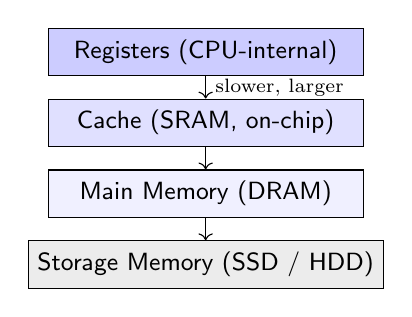
\begin{tikzpicture}[
  level/.style={draw, rectangle, minimum width=4cm, minimum height=0.6cm,
                font=\small\sffamily, align=center},
  every node/.style={anchor=center}
]
  \node[level, fill=blue!20] (reg)  at (0,0)    {Registers (CPU-internal)};
  \node[level, fill=blue!12] (cache) at (0,-0.9)  {Cache (SRAM, on-chip)};
  \node[level, fill=blue!6]  (mm)   at (0,-1.8)  {Main Memory (DRAM)};
  \node[level, fill=gray!15] (stor) at (0,-2.7)  {Storage Memory (SSD / HDD)};
  \draw[->] (reg)  -- node[right,font=\scriptsize]{slower, larger} (cache);
  \draw[->] (cache)-- (mm);
  \draw[->] (mm)   -- (stor);
\end{tikzpicture}
\end{center}

\subsection{CPU Memory Access Sequence}
\label{sec:cpu-access}

When the CPU needs a piece of data it always queries the nearest memory level first:

\begin{enumerate}
  \item The CPU sends a request to the cache.
  \item \textbf{Cache hit}: the data is present — cache returns it immediately. \emph{(Best case.)}
  \item \textbf{Cache miss}: the data is absent — the CPU queries main memory.
  \item If the data is also absent from main memory, a further request goes to disk (storage memory). \emph{(Worst case.)}
  \item Once the data is located at any level, the required data \emph{and a block of its neighbours} are loaded into cache (exploiting spatial locality).
\end{enumerate}

\begin{keyresult}[title={Key Result: Cache as a Buffer}]
  Cache hides the latency of main memory from the CPU. The entire effectiveness of cache rests on the \emph{Principle of Locality}: programs tend to access the same data and nearby data repeatedly, so a small cache can serve a large fraction of all memory requests.
\end{keyresult}

% ────────────────────────────────────────────────────────────────────────────
\section{Principle of Locality}
\label{sec:locality}
% ────────────────────────────────────────────────────────────────────────────

\begin{definition}[Principle of Locality]
  \label{def:locality}
  Programs exhibit \emph{locality}: once a byte of code or data is accessed, it is highly probable that nearby bytes (in address space) or the \emph{same} byte (over time) will be accessed soon.
\end{definition}

There are two complementary types:

\begin{description}
  \item[\textbf{Spatial Locality}] Code and data that reside at \emph{nearby addresses} are likely to be accessed together. This justifies fetching data in \emph{blocks} rather than individual bytes: when a miss occurs, the entire block containing the needed byte is copied into cache, so subsequent accesses to adjacent addresses are cache hits.

  \item[\textbf{Temporal Locality}] Recently accessed code or data is likely to be accessed \emph{again soon}. This governs cache \emph{replacement policy}: when a block must be evicted to make room, the least recently used block is evicted (it is the least likely to be needed again).
\end{description}

\begin{example}[Locality in a Loop]
  \label{ex:locality-loop}
  Consider the loop:
  \begin{lstlisting}[language=C]
for (i = 0; i < 10; i++)
    y[i] = a[i] * x[i];
  \end{lstlisting}
  \begin{itemize}
    \item \textbf{Spatial}: Accessing \texttt{a[0]} makes it very likely that \texttt{a[1]}, \texttt{a[2]}, \ldots\ will be accessed next — justifying the block-fetch strategy.
    \item \textbf{Temporal}: The loop body is executed 10 times, so the same instructions are fetched from cache on each iteration rather than from main memory.
  \end{itemize}
\end{example}

\begin{examtip}[title={Exam Tip: Transfer is Always in Blocks}]
  Data transfer between main memory and cache always happens in \emph{whole blocks} (cache lines), never one byte at a time. This is a direct consequence of spatial locality. Do not confuse the \emph{block size} (e.g.\ 4 bytes or 16 bytes) with the individual byte requested by the CPU.
\end{examtip}

% ────────────────────────────────────────────────────────────────────────────
\section{Cache Mapping Scheme}
\label{sec:cache-mapping}
% ────────────────────────────────────────────────────────────────────────────

The \emph{cache mapping scheme} determines which cache location a given main memory block maps to. Three schemes exist: Direct Mapped, Set Associative, and Fully Associative. This course covers only \textbf{Direct Mapped Cache}; the other two are treated in Advanced Computer Architecture.

\subsection{Key Terminology}
\label{sec:cache-terms}

\begin{description}
  \item[\textbf{Cache Block} (Cache Line)] The basic unit of storage in the cache. A cache with block size $B$ bytes holds $B$ bytes in each block. All transfers between main memory and cache move one whole block.
  \item[\textbf{Block Index} (Cache Block Number)] The integer index $0, 1, \ldots, N-1$ identifying which block of the $N$-block cache is being referred to.
  \item[\textbf{Offset}] The byte position within a block, ranging from $0$ to $B-1$. The number of bits required for the offset field is $\log_2 B$.
  \item[\textbf{Tag}] Bits from the main memory address left over after allocating for Block Index and Offset. The tag uniquely identifies which main memory block occupies a given cache block.
\end{description}

\subsection{Direct Mapped Cache}
\label{sec:direct-mapped}

In a direct-mapped cache with $N$ cache blocks, main memory block number $X$ (not the full address, but the block number) maps deterministically to cache block:
\[
  Y = X \bmod N.
\]
This gives each main memory block a \emph{fixed} home in the cache. If two frequently accessed blocks share the same home, they thrash each other out of cache (a limitation of direct mapping).

\subsubsection{Address Field Partitioning (TAG : BLK : OFFSET)}
\label{sec:tag-blk-offset}

Every main memory address is partitioned into three contiguous fields, always computed from the \emph{least significant end}:

\begin{enumerate}
  \item \textbf{OFFSET} (LSBs): $\log_2(\text{block size in bytes})$ bits.
  \item \textbf{BLK} (middle bits): $\log_2(\text{number of cache blocks})$ bits.
  \item \textbf{TAG} (MSBs): remaining bits $= \text{total address bits} - \text{BLK bits} - \text{OFFSET bits}$.
\end{enumerate}

\begin{center}
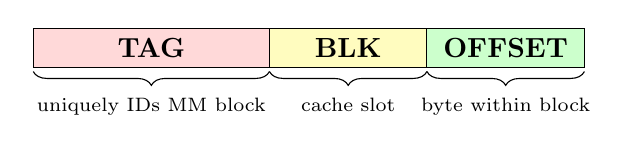
\begin{tikzpicture}
  \draw[fill=red!15]    (0,0) rectangle (3.0,0.5) node[midway]{\textbf{TAG}};
  \draw[fill=yellow!25] (3.0,0) rectangle (5.0,0.5) node[midway]{\textbf{BLK}};
  \draw[fill=green!20]  (5.0,0) rectangle (7.0,0.5) node[midway]{\textbf{OFFSET}};
  \draw[decorate, decoration={brace,amplitude=5pt,mirror}]
      (0,-0.05) -- (3.0,-0.05) node[midway,below=6pt]{\scriptsize uniquely IDs MM block};
  \draw[decorate, decoration={brace,amplitude=5pt,mirror}]
      (3.0,-0.05) -- (5.0,-0.05) node[midway,below=6pt]{\scriptsize cache slot};
  \draw[decorate, decoration={brace,amplitude=5pt,mirror}]
      (5.0,-0.05) -- (7.0,-0.05) node[midway,below=6pt]{\scriptsize byte within block};
\end{tikzpicture}
\end{center}

\begin{warning}[title={Warning: Always Work in Binary}]
  The TAG:BLK:OFFSET partitioning is a \emph{binary field split}. Always convert the main memory address to binary before applying the partition — operating in hexadecimal leads to systematic errors because the field boundaries do not generally fall on hex digit boundaries.
\end{warning}

\subsubsection{Worked Example: Address Mapping}
\label{ex:cache-mapping}

\begin{example}[Finding the Cache Block for a Given Address]
  \label{ex:cache-map1}
  \textbf{System parameters:}
  \begin{itemize}
    \item Main memory size: 64\,KB $= 2^{16}$ bytes $\Rightarrow$ 16-bit addresses.
    \item Cache size: 256\,bytes.
    \item Cache block size: 16\,bytes.
  \end{itemize}

  \textbf{Step 1 — Derive field widths.}
  \begin{align*}
    \text{OFFSET bits} &= \log_2(16) = 4. \\
    \text{Number of cache blocks} &= 256 / 16 = 16. \\
    \text{BLK bits} &= \log_2(16) = 4. \\
    \text{TAG bits} &= 16 - 4 - 4 = 8.
  \end{align*}
  The mapping format is \textbf{8 : 4 : 4}.

  \textbf{Step 2 — Map address \texttt{0x1106}.}
  \[
    \texttt{0x1106} = (0001\ 0001\ 0000\ 0110)_2.
  \]
  Applying the 8:4:4 split:
  \[
    \underbrace{0001\ 0001}_{\text{TAG} = \texttt{0x11}}\ \underbrace{0000}_{\text{BLK} = 0}\ \underbrace{0110}_{\text{OFFSET} = 6}.
  \]
  The byte at \texttt{0x1106} will be stored in \textbf{cache block 0}, tagged with \texttt{0x11}, at byte offset 6 within the block.
\end{example}

\subsection{Cache Hit and Miss Detection}
\label{sec:hit-miss}

When the CPU requests main memory address $A$:
\begin{enumerate}
  \item Partition $A$ into TAG, BLK, OFFSET using the mapping format.
  \item Go to cache block \emph{BLK}.
  \item Compare the stored tag of that cache block with the TAG field of $A$.
  \item \textbf{Cache Hit}: tags match — the correct block is in cache. Retrieve the byte at position \emph{OFFSET}.
  \item \textbf{Cache Miss}: tags differ — the block needed is not present. The corresponding main memory block is fetched and written into cache block \emph{BLK}, overwriting whatever was there. Then the CPU retrieves the byte.
\end{enumerate}

\begin{example}[Cache Hit and Miss]
  \label{ex:hit-miss}
  Using the same system from Example~\ref{ex:cache-map1} (mapping format 4:2:2 in the lecture's smaller example with 8-bit addresses):

  \begin{itemize}
    \item \textbf{Request \texttt{0x8C}}: Binary \texttt{1000 11 00} $\Rightarrow$ TAG = \texttt{0x8}, BLK = 3, OFFSET = 0. Cache block 3 holds tag \texttt{0x8}: \emph{match} $\Rightarrow$ \textbf{Cache Hit}.
    \item \textbf{Request \texttt{0x84}}: Binary \texttt{1000 01 00} $\Rightarrow$ TAG = \texttt{0x8}, BLK = 1, OFFSET = 0. Cache block 1 holds tag \texttt{0x9}: \emph{mismatch} $\Rightarrow$ \textbf{Cache Miss}. The MM block containing \texttt{0x84}--\texttt{0x87} is fetched into cache block 1.
  \end{itemize}
\end{example}

% ────────────────────────────────────────────────────────────────────────────
\section{Cache Replacement Policy}
\label{sec:cache-replacement}
% ────────────────────────────────────────────────────────────────────────────

For direct-mapped cache the replacement destination is uniquely determined by the block number ($X \bmod N$), so no policy decision is needed. In \emph{set-associative} and \emph{fully associative} caches (covered in Advanced Computer Architecture), there is a choice of which existing block to evict when all candidate slots are occupied. Two common policies are:

\begin{description}
  \item[\textbf{Least Recently Used (LRU)}] Evicts the block that has been unused for the longest time. Conforms closely to temporal locality and achieves high efficiency; however, it requires maintaining a per-block access-history record, adding hardware cost and slowing down the cache.
  \item[\textbf{First-In, First-Out (FIFO)}] Evicts the block that has been in cache the longest, regardless of how recently it was accessed. Simpler to implement than LRU but can evict frequently-used blocks, resulting in lower efficiency.
\end{description}

% ────────────────────────────────────────────────────────────────────────────
\section{Cache Write Policy}
\label{sec:cache-write}
% ────────────────────────────────────────────────────────────────────────────

Cache design so far has focused on read operations. Write operations require additional policy decisions. A cache block that the CPU has written to but whose corresponding main memory block has \emph{not} yet been updated is called a \textbf{Dirty Block}.

\subsection{Write-Hit Policies}
\label{sec:write-hit}

A \emph{write hit} occurs when the CPU writes to an address currently present in cache.

\begin{description}
  \item[\textbf{Write-Through}] The CPU writes simultaneously to both the cache block and the corresponding main memory location on every write. Guarantees cache–memory \emph{coherence} at all times, but generates heavy traffic on the system bus (memory bus) because every write propagates to main memory.

  \item[\textbf{Write-Back} (Copyback)] The CPU writes only to the cache block. The main memory is updated \emph{only when the dirty cache block is evicted}. Reduces bus traffic significantly, but the cache module must track whether each block is dirty (using a \emph{dirty bit}) to know whether a write-back is required on eviction. There is a transient window of \emph{incoherence} between cache and main memory.
\end{description}

\subsection{Write-Miss Policies}
\label{sec:write-miss}

A \emph{write miss} occurs when the CPU writes to an address \emph{not} currently in cache.

\begin{description}
  \item[\textbf{Write-Allocate} (Fetch-on-Write)] The corresponding main memory block is first loaded into cache, then the write is performed on the cached copy (following the write-hit policy). Future accesses to the same block are likely to be cache hits. Pairs naturally with Write-Back.
  \item[\textbf{Write-No-Allocate}] The CPU writes directly to main memory without bringing the block into cache. The cache is not updated. Simpler, but subsequent accesses to the same block will still miss. Pairs naturally with Write-Through.
\end{description}

\begin{keyresult}[title={Key Result: Write Policy Combinations}]
  In practice, the two commonly paired combinations are:
  \begin{itemize}
    \item \textbf{Write-Back + Write-Allocate}: fewer bus transactions, more complex dirty-bit management.
    \item \textbf{Write-Through + Write-No-Allocate}: simpler coherence, higher bus traffic.
  \end{itemize}
\end{keyresult}

% ────────────────────────────────────────────────────────────────────────────
\section{Effective Access Time (EAT)}
\label{sec:eat}
% ────────────────────────────────────────────────────────────────────────────

\begin{definition}[Effective Access Time]
  \label{def:eat}
  The \emph{effective access time} (EAT) is the weighted average memory access time experienced by the CPU, taking into account both the probability of a cache hit and the access times of each memory level.
\end{definition}

Let:
\begin{itemize}
  \item $H$ = cache hit rate (fraction of accesses that are cache hits, $0 \le H \le 1$).
  \item $\text{Access}_C$ = cache access time.
  \item $\text{Access}_{MM}$ = main memory access time.
\end{itemize}

Assuming cache and main memory are accessed \emph{sequentially} (i.e., on a miss, the cache is checked first, then main memory — accesses do not overlap):

\begin{equation}
  \text{EAT} = H \cdot \text{Access}_C + (1-H)\cdot(\text{Access}_C + \text{Access}_{MM}).
  \label{eq:eat}
\end{equation}

This simplifies to:
\[
  \text{EAT} = \text{Access}_C + (1-H)\cdot \text{Access}_{MM}.
\]

\begin{warning}[title={Warning: EAT Formula Applies to READ Only}]
  Equation~\eqref{eq:eat} applies only to \emph{read} operations. Write operations are more complex because the effective penalty depends on the combination of write-through/write-back and write-allocate/write-no-allocate policies in use.
\end{warning}

\begin{example}[EAT Calculation]
  \label{ex:eat}
  A system has main memory access time $200$\,ns, cache access time $10$\,ns, and a cache hit rate of $99\%$.

  \[
    \text{EAT} = 0.99 \times 10\text{\,ns} + 0.01 \times (10 + 200)\text{\,ns}
               = 9.9\text{\,ns} + 2.1\text{\,ns} = 12\text{\,ns}.
  \]

  Without cache, every access would take $200$\,ns. The cache reduces the effective access time to $12$\,ns — a $16.7\times$ improvement. This illustrates how a cache with a high hit rate and a $20\times$ speed advantage can dominate the overall EAT.
\end{example}

\begin{examtip}[title={Exam Tip: EAT Steps}]
  (1) Identify $H$, $\text{Access}_C$, and $\text{Access}_{MM}$. (2) Apply Equation~\eqref{eq:eat}. (3) Confirm the assumption that accesses are \emph{sequential} (the problem should state this). (4) The miss penalty is $\text{Access}_C + \text{Access}_{MM}$, \emph{not} just $\text{Access}_{MM}$, because the CPU still pays the cache access time even on a miss.
\end{examtip}

% ════════════════════════════════════════════════════════════════════════════
\chapter{Virtual Memory Management}
\label{chap:virtual-memory}
% ════════════════════════════════════════════════════════════════════════════

\section{Memory Address Space}
\label{sec:address-space}

\begin{definition}[Address Space]
  \label{def:address-space}
  An \emph{address space} is a range of discrete addresses corresponding to a physical or logical entity — for example, the virtual address space of a program, the physical address space of main memory, or the logical block address space of a hard disk.
\end{definition}

Different entities within a computer each maintain their own address space with their own addressing scheme:

\begin{itemize}
  \item \textbf{Program (Virtual Address Space)}: Addresses generated by the compiler and assigned by the OS. Each program has its own independent virtual address space.
  \item \textbf{System/Main Memory (Physical Address Space)}: Addresses of actual DRAM locations.
  \item \textbf{Storage Memory (Logical Block Addressing, LBA)}: Addresses of 512-byte sectors on an HDD or SSD (see Chapter~9).
\end{itemize}

The same piece of data (e.g.\ a video file) may be stored at \emph{different addresses} in each of these spaces simultaneously. \emph{Address translation} — performed by the Operating System (OS) — bridges these different address spaces transparently.

\subsection{Virtual vs.\ Physical Address}
\label{sec:virtual-vs-physical}

\begin{itemize}
  \item The addresses a program uses are called \textbf{virtual addresses}. They are generated by the compiler and allocated by the OS.
  \item The addresses of actual locations in main memory are called \textbf{physical addresses} (also called ``main memory addresses'' or ``system memory addresses'' — all synonymous in this course).
  \item Virtual addresses are typically \emph{different} from the physical addresses where the data actually resides.
  \item The OS is responsible for translating virtual to physical addresses. This translation is implemented in hardware and/or software.
\end{itemize}

% ────────────────────────────────────────────────────────────────────────────
\section{Virtual Memory Management}
\label{sec:vmm}
% ────────────────────────────────────────────────────────────────────────────

The OS manages virtual memory by:
\begin{enumerate}
  \item Maintaining a \emph{per-program} virtual address space. Each running program sees its own private virtual memory, independent of other programs.
  \item Loading only the \emph{subset} of a program's code and data that is required at any given moment into physical main memory. The complete program resides in storage memory (HDD/SSD).
  \item Performing \emph{address translation} from virtual to physical addresses on every memory access.
\end{enumerate}

\subsection{Advantages of Virtual Memory}
\label{sec:vmm-advantages}

\begin{itemize}
  \item \textbf{Isolation and Protection}: Each program's virtual address space is isolated from every other program's. The OS can prevent one program from reading or corrupting another program's memory.
  \item \textbf{Efficient Sharing}: Multiple programs share the same physical memory simultaneously. The OS multiplexes physical memory across programs, only keeping the actively used portions of each in RAM.
  \item \textbf{Programs Larger than Physical Memory}: The OS can run programs whose total combined size exceeds physical memory by swapping pages between main memory and storage memory as needed.
  \item \textbf{Contiguous Logical View}: The OS maps virtual address space to \emph{fragmented} physical frames in a way that appears contiguous to the program. This greatly simplifies programming — the programmer need not manage physical memory fragmentation.
\end{itemize}

% ────────────────────────────────────────────────────────────────────────────
\section{Paging: Address Mapping Scheme}
\label{sec:paging}
% ────────────────────────────────────────────────────────────────────────────

Two address mapping schemes exist in industry: \textbf{Paging} (fixed-size blocks) and \textbf{Segmentation} (variable-size blocks). This course covers \textbf{paging with a single-level page table} only.

\begin{definition}[Page and Frame]
  \label{def:page-frame}
  In a paging system:
  \begin{itemize}
    \item The virtual address space is divided into equal-sized units called \textbf{pages}.
    \item The physical address space is divided into equal-sized units called \textbf{frames}.
    \item Page size $\equiv$ Frame size (always, by definition).
  \end{itemize}
  The OS maps each virtual page to a physical frame. The mapping is recorded in a data structure called the \textbf{Page Table}.
\end{definition}

\subsection{The Page Table}
\label{sec:page-table}

Each entry in the page table contains at minimum:

\begin{center}
\renewcommand{\arraystretch}{1.3}
\begin{tabularx}{\linewidth}{clX}
  \toprule
  \textbf{Field} & \textbf{Meaning} & \textbf{Note} \\
  \midrule
  Page \# & Virtual page number & Index into the table \\
  Frame \# & Physical frame the page is mapped to & Used in address translation \\
  Valid Bit (VB) & 1 = page is currently in physical memory & 0 = page must be fetched from storage \\
  \bottomrule
\end{tabularx}
\end{center}

If VB = 1, the page's data is in the physical frame given by Frame \#. If VB = 0, a \textbf{page fault} is generated — the OS must load the required page from storage memory into an available physical frame, update the page table, and retry the memory access.

% ────────────────────────────────────────────────────────────────────────────
\section{Virtual-to-Physical Address Translation}
\label{sec:addr-translation}
% ────────────────────────────────────────────────────────────────────────────

The process of translating a virtual address to a physical address in a paging system is entirely analogous to the TAG:BLK:OFFSET split used in cache mapping (Chapter~\ref{chap:cache}), but the two fields here are \textbf{Virtual Page Number} and \textbf{Page Offset}.

\subsection{Address Field Partitioning}

\begin{enumerate}
  \item Convert the virtual address to binary.
  \item \textbf{Offset field} (LSBs): $\log_2(\text{page size in bytes})$ bits. \emph{The offset is preserved unchanged in the physical address.}
  \item \textbf{Virtual Page Number} (VPN, remaining MSBs): used to index the page table.
\end{enumerate}

The physical address is formed by:
\begin{center}
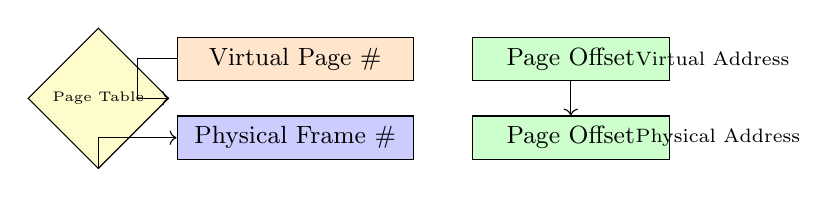
\begin{tikzpicture}
  \node[draw, fill=orange!20, minimum width=3cm, minimum height=0.55cm, font=\small]
      (vpn)  at (0,1)    {Virtual Page \#};
  \node[draw, fill=green!20,  minimum width=2.5cm, minimum height=0.55cm, font=\small]
      (off)  at (3.5,1)  {Page Offset};
  \node[font=\small\bfseries] at (1.75,1) {};

  \node[draw, fill=blue!20, minimum width=3cm, minimum height=0.55cm, font=\small]
      (fpn)  at (0,0)    {Physical Frame \#};
  \node[draw, fill=green!20,  minimum width=2.5cm, minimum height=0.55cm, font=\small]
      (off2) at (3.5,0)  {Page Offset};

  \node[draw, diamond, fill=yellow!20, minimum size=0.8cm, font=\tiny]
      (pt)  at (-2.5,0.5) {Page Table};

  \draw[->] (vpn.west) -- ++(-0.5,0) |- (pt.east);
  \draw[->] (pt.south) |- (fpn.west);
  \draw[->] (off.south) -- (off2.north);

  \node[font=\scriptsize, right] at (4.2,1) {Virtual Address};
  \node[font=\scriptsize, right] at (4.2,0) {Physical Address};
\end{tikzpicture}
\end{center}

The offset bits pass through unchanged. Only the upper bits (VPN) are replaced by the corresponding Physical Frame Number read from the page table.

\begin{keyresult}[title={Key Result: Address Translation Steps}]
  \begin{enumerate}
    \item Convert virtual address to binary.
    \item Compute offset bits: $\log_2(\text{page size})$.
    \item Extract VPN from the upper bits; extract offset from the lower bits.
    \item Look up VPN in the page table:
    \begin{itemize}
      \item Valid Bit = 1: replace VPN with the Frame \# to form the physical address.
      \item Valid Bit = 0: \textbf{page fault} — OS loads the page from storage, updates the table, retries.
    \end{itemize}
    \item Physical address = $[\text{Frame \#}][\text{Offset}]$ concatenated in binary.
  \end{enumerate}
\end{keyresult}

\subsection{Worked Example: Paging System}
\label{sec:paging-example}

\begin{example}[Address Translation in an 8K/4K System]
  \label{ex:paging1}
  \textbf{System:} Virtual address space = 8\,KB, Physical address space = 4\,KB, Page size = 1\,KB.

  \textbf{Derived parameters:}
  \begin{align*}
    \text{Offset bits} &= \log_2(1024) = 10. \\
    \text{Virtual address bits} &= \log_2(8192) = 13. \\
    \text{Physical address bits} &= \log_2(4096) = 12. \\
    \text{VPN bits} &= 13 - 10 = 3 \Rightarrow 2^3 = 8 \text{ virtual pages.} \\
    \text{Frame \# bits} &= 12 - 10 = 2 \Rightarrow 2^2 = 4 \text{ physical frames.}
  \end{align*}

  Suppose the page table is:

  \begin{center}
  \renewcommand{\arraystretch}{1.2}
  \begin{tabular}{ccc}
    \toprule
    \textbf{Page \#} & \textbf{Frame \#} & \textbf{Valid Bit} \\
    \midrule
    0 & -- & 0 \\
    1 & 3  & 1 \\
    2 & 0  & 1 \\
    3 & -- & 0 \\
    4 & -- & 0 \\
    5 & 1  & 1 \\
    6 & 2  & 1 \\
    7 & -- & 0 \\
    \bottomrule
  \end{tabular}
  \end{center}

  \textbf{Translate virtual address \texttt{0x1553}:}
  \[
    \texttt{0x1553} = (1\,0101\,0101\,0011)_2.
  \]
  VPN (upper 3 bits) = $101_2 = 5$. Offset (lower 10 bits) = $01\,0101\,0011_2$.

  Page 5 has Valid Bit = 1 and maps to Frame 1.

  Physical address = $01_2 \| 01\,0101\,0011_2 = (01\,0101\,0101\,0011)_2 = \texttt{0x0553}$.

  \textbf{Translate virtual address \texttt{0x0FA0}:}
  \[
    \texttt{0x0FA0} = (0\,1111\,1010\,0000)_2.
  \]
  VPN = $011_2 = 3$. Page 3 has Valid Bit = 0.

  $\Rightarrow$ \textbf{Page Fault.} The OS must load virtual page 3 from storage memory into a free physical frame, update the page table, and re-execute the access.
\end{example}

\begin{warning}[title={Warning: Page Fault $\ne$ Error}]
  A page fault is \emph{not} a program error. It is a normal OS mechanism: the required page simply is not in main memory at that moment. The OS services the fault transparently by loading the page from disk and resuming the program.
\end{warning}

% ────────────────────────────────────────────────────────────────────────────
\section{Integration of Cache and Virtual Memory}
\label{sec:cache-vm-integration}
% ────────────────────────────────────────────────────────────────────────────

A real system implements \emph{both} cache and virtual memory simultaneously. When the CPU accesses a virtual address, the typical sequence (assuming the cache uses \emph{physical addresses}) is:

\begin{enumerate}
  \item Translate the virtual address to a physical address using the page table.
  \item Check the cache using the physical address (cache hit or miss evaluation using the TAG:BLK:OFFSET scheme from Chapter~\ref{chap:cache}).
  \item On a cache hit: retrieve data from cache.
  \item On a cache miss: fetch the block from main memory into cache, then return the data.
\end{enumerate}

If the cache uses \emph{virtual addresses} for indexing, the CPU queries the cache \emph{before} address translation, but must still perform translation on a cache miss to fetch data from main memory.

% ────────────────────────────────────────────────────────────────────────────
\section{Translation Lookaside Buffer (TLB)}
\label{sec:tlb}
% ────────────────────────────────────────────────────────────────────────────

\begin{definition}[TLB]
  \label{def:tlb}
  A \emph{Translation Lookaside Buffer} (TLB) is a small, fast cache for page table entries, residing inside the processor. It stores a subset of the most recently or frequently used virtual-page-to-physical-frame mappings.
\end{definition}

The page table can be several megabytes in size and must reside in main memory, making every address translation an expensive main-memory access. The TLB avoids this overhead: if the required mapping is in the TLB (a \textbf{TLB hit}), the physical frame number is obtained at internal-memory speed, far faster than a main memory access.

\begin{warning}[title={Warning: TLB $\ne$ Data Cache}]
  The TLB caches \emph{address translation information} (VPN $\mapsto$ Frame \#) only. It does not store program code or data. The data cache (Chapter~\ref{chap:cache}) stores actual code and data. They are separate hardware structures serving different purposes.
\end{warning}

\subsection{TLB Lookup: Three Scenarios}
\label{sec:tlb-scenarios}

Starting from a virtual address:

\begin{description}
  \item[\textbf{TLB Hit}] The VPN is found in the TLB. The corresponding Frame \# is read directly, the physical address is formed, and data is accessed. Fast path — no main memory access needed for translation.
  \item[\textbf{TLB Miss (Page Table Hit)}] The VPN is not in the TLB but is found with Valid Bit = 1 in the main-memory page table. The Frame \# is obtained from main memory, the TLB is updated with this entry, and the physical address is formed. One extra main memory access for translation.
  \item[\textbf{Page Fault}] The VPN is neither in the TLB nor valid in the page table. The OS loads the required page from storage into a free physical frame, updates the page table, and optionally updates the TLB. Slowest path — disk access required.
\end{description}

\begin{center}
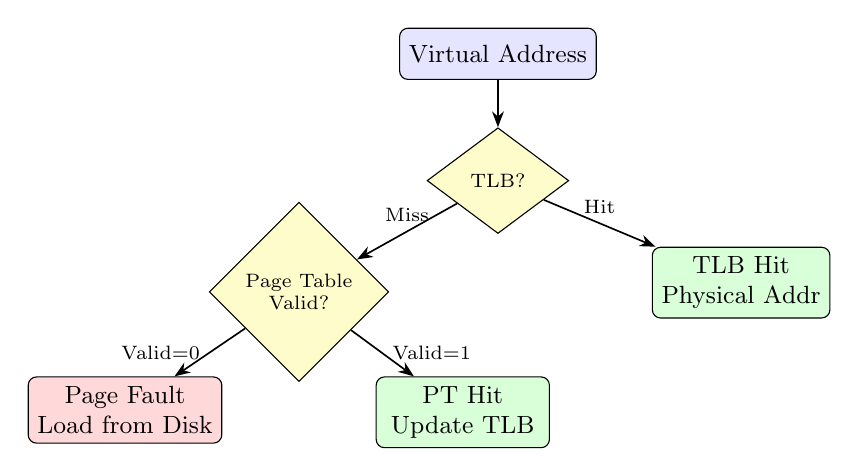
\begin{tikzpicture}[
  node distance=0.5cm and 1.5cm,
  box/.style={draw, rectangle, rounded corners=3pt, minimum height=0.65cm,
              minimum width=2.2cm, align=center, font=\small},
  dec/.style={draw, diamond, minimum height=0.7cm, minimum width=1.8cm,
              align=center, font=\scriptsize},
  arr/.style={-Stealth, semithick}
]
  \node[box, fill=blue!10]  (va)  {Virtual Address};
  \node[dec, fill=yellow!20, below=0.6cm of va] (tlb) {TLB?};
  \node[box, fill=green!15, below right=0.5cm and 1.5cm of tlb] (hit) {TLB Hit\\Physical Addr};
  \node[dec, fill=yellow!20, below left=0.5cm and 1.5cm of tlb]  (pt)  {Page Table\\Valid?};
  \node[box, fill=green!15, below right=0.5cm and 0.4cm of pt]  (pthit) {PT Hit\\Update TLB};
  \node[box, fill=red!15,   below left=0.5cm and 0.4cm of pt]   (pf)  {Page Fault\\Load from Disk};

  \draw[arr] (va)   -- (tlb);
  \draw[arr] (tlb)  -- node[above,font=\scriptsize]{Hit} (hit);
  \draw[arr] (tlb)  -- node[above,font=\scriptsize]{Miss} (pt);
  \draw[arr] (pt)   -- node[right,font=\scriptsize]{Valid=1} (pthit);
  \draw[arr] (pt)   -- node[left, font=\scriptsize]{Valid=0} (pf);
\end{tikzpicture}
\end{center}

\begin{keyresult}[title={Key Result: TLB as a Cache for Page Table}]
  The TLB functions like a cache (Chapter~\ref{chap:cache}) but for page table entries rather than data. A high TLB hit rate means virtual-to-physical translation is performed almost entirely at processor speed, eliminating the cost of main-memory page table lookups for the vast majority of accesses.
\end{keyresult}

\begin{examtip}[title={Exam Tip: Three-Level Address Lookup Summary}]
  Know all three access paths (TLB Hit / TLB Miss with Page Table Hit / Page Fault) and be able to state what happens at each step. Pay attention to whether the TLB is updated after a TLB miss — this depends on the VM design and may be tested explicitly.
\end{examtip}

% ════════════════════════════════════════════════════════════════════════════
\chapter{Communication and User Interface}
\label{chap:comm-ui}
% ════════════════════════════════════════════════════════════════════════════

This chapter provides a general overview of the common wired and wireless communication technologies used in computers---specifically USB and HDMI for wired, and Wi-Fi and Bluetooth for wireless---as well as the user-interface devices that transfer real-world data into and out of the digital domain: keyboards, mice, capacitive touch screens, cameras, microphones, displays, and audio speakers. The discussion here is intentionally at a conceptual level; detailed protocol-layer analysis is beyond the scope of SC1006.

% ════════════════════════════════════════════════════════════════════════════
\section{Wired Communication Interfaces}
\label{sec:wired-comm}
% ════════════════════════════════════════════════════════════════════════════

\subsection{Universal Serial Bus (USB)}
\label{sec:usb}

\begin{definition}[Universal Serial Bus]
  \label{def:usb}
  The \emph{Universal Serial Bus (USB)} is a serial bus standard designed to provide a single, unified interface for connecting computer peripheral devices---keyboards, mice, printers, disk drives, network adapters, digital cameras, and many others. It effectively replaced a large number of legacy interface buses such as the RS-232 serial (COM) port and the parallel printer port.
\end{definition}

USB has evolved substantially since its introduction. USB~1.0 supported a maximum transfer rate of 12\,Mbps; the latest USB~3.2 standard supports up to 20\,Gbps. The basic USB connector has four pins: VBUS (+5\,V power supply), Data+ and Data$-$ (the differential data pair), and Ground.

\subsubsection{USB Topology and Host Model}

USB employs a \emph{tiered-star topology}. At the centre of every star sits the \textbf{USB Host}, which is typically integrated into the computer's chipset. Peripheral devices (mice, keyboards, etc.) connect either directly to the Host or indirectly through intermediate \textbf{USB Hub} devices.

\begin{figure}[h]
\centering
\resizebox{0.85\linewidth}{!}{%
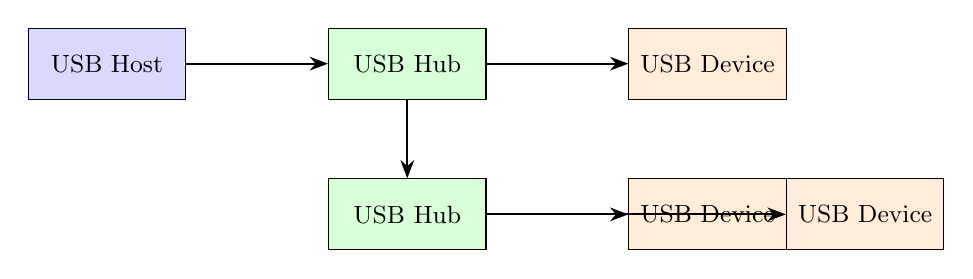
\begin{tikzpicture}[
    block/.style={draw, rectangle, minimum width=2cm, minimum height=0.9cm, align=center, font=\small},
    arr/.style={-{Stealth}, thick}
  ]
  \node[block, fill=blue!15] (host) {USB Host};
  \node[block, fill=green!15, right=1.8cm of host] (hub1) {USB Hub};
  \node[block, fill=orange!15, right=1.8cm of hub1] (dev1) {USB Device};
  \node[block, fill=green!15, below=1cm of hub1] (hub2) {USB Hub};
  \node[block, fill=orange!15, right=1.8cm of hub2] (dev2) {USB Device};
  \node[block, fill=orange!15, right=3.8cm of hub2] (dev3) {USB Device};

  \draw[arr] (host) -- (hub1);
  \draw[arr] (hub1) -- (dev1);
  \draw[arr] (hub1) -- (hub2);
  \draw[arr] (hub2) -- (dev2);
  \draw[arr] (hub2) -- (dev3);
\end{tikzpicture}%
}
\caption{USB tiered-star topology. Hubs extend the bus; all transactions are initiated by the Host.}
\label{fig:usb-topology}
\end{figure}

Several important properties follow from the host-centric design:

\begin{itemize}
  \item All data transactions are \emph{initiated by the USB Host}. Data flowing into the Host is called an \textbf{IN} transaction; data flowing out is an \textbf{OUT} transaction.
  \item The Host assigns a unique address to each connected device so that it can direct traffic to the correct peripheral.
  \item Power can be supplied by the Host or Hub (\emph{bus-powered}), or the device may have its own supply (\emph{self-powered}).
\end{itemize}

\subsubsection{USB Enumeration and Device Classes}

When a USB device is first connected, it undergoes an \emph{enumeration} process: the device and the Host exchange capability and requirement information---for example, the device reports its Vendor~ID, Product~ID, device class, and required bandwidth. The Host cannot communicate with the device until enumeration is complete.

After enumeration the Host checks whether it has a suitable \emph{device driver} matching the USB \textbf{device class} that the peripheral belongs to. Common USB device classes include:

\begin{itemize}
  \item \textbf{Human Interface Device (HID)} --- used for mice and keyboards.
  \item \textbf{Communication Device Class (CDC)} --- used to implement a Virtual COM Port (e.g.\ Arduino boards, MSP432 LaunchPads).
  \item \textbf{Mass Storage Class (MSC)} --- used to interface with external USB HDDs and SSDs.
  \item \textbf{USB Audio Class} --- used to stream audio to USB headsets and microphones.
\end{itemize}

\begin{examtip}[title={Exam Tip: USB Host-Initiated Transactions}]
  Remember that \emph{all} USB data transactions are initiated by the Host, not the peripheral device. The Host polls peripherals according to their endpoint descriptors; even an ``interrupt'' transfer type is actually Host-polled at a guaranteed frequency.
\end{examtip}

% ────────────────────────────────────────────────────────────────────────────
\subsection{High-Definition Multimedia Interface (HDMI)}
\label{sec:hdmi}

\begin{definition}[HDMI]
  \label{def:hdmi}
  \emph{HDMI (High-Definition Multimedia Interface)} is a proprietary audio/video interface for transmitting uncompressed video data and compressed or uncompressed digital audio data from a source device (e.g.\ a display controller in a computer) to a compatible receiver such as a monitor, digital television, or digital audio device.
\end{definition}

Beyond audio/video transport, HDMI includes a \textbf{CEC (Consumer Electronics Control)} capability that allows connected HDMI devices to control each other, enabling the user to operate multiple devices with a single remote control.

Three commonly used HDMI connector types exist: \textbf{Type~A} (standard), \textbf{Type~C} (Mini), and \textbf{Type~D} (Micro). The original HDMI~v1.0/1.1 specification supported a transfer rate of 3.96\,Gbps, sufficient for 1080p video at 60\,fps. The latest HDMI~v2.1 achieves 42.6\,Gbps, enabling 8K-resolution video.


% ════════════════════════════════════════════════════════════════════════════
\section{Wireless Communication}
\label{sec:wireless-comm}
% ════════════════════════════════════════════════════════════════════════════

\subsection{ISM Radio-Frequency Bands}
\label{sec:ism-band}

Wireless standards used in computing almost universally operate within the \emph{Industrial, Scientific and Medical (ISM)} radio-frequency bands---a set of ``royalty-free'' frequency allocations. Some ISM bands are global (available worldwide) while others are restricted to specific geographical regions. The two most important worldwide ISM bands are \textbf{2.4\,GHz} and \textbf{5.8\,GHz}. Multiple wireless technologies---including Wi-Fi, Bluetooth, ZigBee, and proprietary low-power radio---all share these bands, which can lead to mutual interference.

\subsection{Wi-Fi (IEEE 802.11)}
\label{sec:wifi}

\begin{definition}[Wi-Fi]
  \label{def:wifi}
  \emph{Wi-Fi} is a family of wireless networking technologies based on the IEEE~802.11 family of standards, commonly known as ``Wireless LAN.'' Wi-Fi operates in the 2.4\,GHz and 5.8\,GHz ISM bands.
\end{definition}

Wi-Fi supports two common topologies:

\begin{itemize}
  \item \textbf{Infrastructure Mode} --- a star topology with an Access Point (AP) or router at the centre, to which all end devices connect.
  \item \textbf{Ad-hoc Mode} --- a peer-to-peer connection between devices with no central access point.
\end{itemize}

The typical Wi-Fi transmission range lies between 20\,m and 150\,m, depending on factors such as transmission frequency, transmission power, and interference. The latest standard, 802.11ax (Wi-Fi~6), achieves transfer rates of up to approximately 10\,Gbps.

\subsection{Bluetooth}
\label{sec:bluetooth}

\begin{definition}[Bluetooth]
  \label{def:bluetooth}
  \emph{Bluetooth} is a short-range wireless standard designed primarily for low-data-rate transmission with an emphasis on low power consumption. It operates in the 2.4\,GHz ISM band and uses a star topology.
\end{definition}

Common Bluetooth applications include wireless headsets, smart wearables, and Bluetooth mice. The maximum transmission range is approximately 100\,m, but devices typically operate at 10--20\,m to minimise power draw. Transfer rates are on the order of Kbps to Mbps.

The Bluetooth standard defines two distinct protocols: \textbf{Bluetooth Classic (BT Classic)} and \textbf{Bluetooth Low Energy (BLE)}. These are based on completely different network-layer protocols and are \emph{not mutually compatible}. However, most modern Bluetooth hosts are ``Dual Mode'' and can connect to both BT Classic and BLE devices.

\subsection{Factors Affecting Wireless Transmission Range}
\label{sec:wireless-range}

Three principal factors govern the effective range of a wireless link:

\begin{enumerate}
  \item \textbf{Transmission power} --- higher power directly extends the range.
  \item \textbf{Transmission frequency} --- higher-frequency signals experience greater attenuation as they propagate through air or other media; all else being equal, a higher-frequency signal has a shorter range than a lower-frequency one.
  \item \textbf{Interference} --- many commonly adopted standards (Wi-Fi, Bluetooth, ZigBee) share the 2.4\,GHz ISM band and can interfere with one another. The closer the transmitters, the stronger the interference. Even household microwave ovens radiate energy in the 2.4\,GHz range.
\end{enumerate}

\subsection{Mitigating Interference}
\label{sec:interference}

The ``2.4\,GHz ISM band'' actually spans a range of frequencies from approximately 2.4 to 2.5\,GHz. The Wi-Fi standard divides this band into sub-bands called \emph{channels}, each 22\,MHz wide. Two common interference-mitigation strategies are:

\begin{itemize}
  \item \textbf{Channel selection} --- choosing a channel different from those used by neighbouring networks to reduce overlap.
  \item \textbf{Frequency hopping} --- continuously hopping from one channel to another so that any given collision affects only a brief portion of the transmission. Bluetooth uses frequency hopping.
\end{itemize}

\begin{keyresult}[title={Key Result: Wireless Range Trade-offs}]
  Higher frequency $\Rightarrow$ higher data rate capability but shorter range due to increased atmospheric attenuation. Higher transmission power extends range but increases energy consumption and potential interference with other devices sharing the same band.
\end{keyresult}


% ════════════════════════════════════════════════════════════════════════════
\section{User Interface Devices --- Input}
\label{sec:ui-input}
% ════════════════════════════════════════════════════════════════════════════

\subsection{Keyboard}
\label{sec:keyboard}

A keyboard is a user input device for transmitting characters (alphabets, numbers, special symbols, etc.) to the computer. Internally, a small microcontroller detects key presses and sends their corresponding \textbf{ASCII codes} to the host PC. Wired keyboards today predominantly use the USB interface and are enumerated as \textbf{HID Keyboard} devices (recall Section~\ref{sec:usb}). Wireless keyboards typically operate in the 2.4\,GHz ISM band using either Bluetooth or a proprietary RF protocol with a USB dongle receiver.

\subsection{Mouse}
\label{sec:mouse}

A mouse is a user pointing device that tracks its position by mechanical or optical means. The core data reported to the PC are the $(x,y)$ coordinate deltas and the states of the left/right buttons; mice with additional features may report scroll-wheel data or extra button states.

Position data is reported to the PC periodically at what is called the \emph{scan/polling rate}. A typical mouse polls at 125\,Hz; gaming mice can reach 1000\,Hz or higher, yielding lower input latency and smoother cursor tracking.

Another key parameter is the \textbf{Dot-Per-Inch (DPI)}, which measures how finely the mouse can track physical movement---a higher DPI means greater sensitivity to small physical movements. Connection technologies mirror those of keyboards (USB HID for wired, 2.4\,GHz ISM for wireless).

\subsection{Capacitive Touch Interface}
\label{sec:capacitive-touch}

\begin{definition}[Capacitive Touch Sensing]
  \label{def:capacitive-touch}
  A \emph{capacitive touch} pad or button is modelled electrically as a capacitor. When a conductive element---such as a human finger---approaches or contacts the pad, the effective capacitance of the system increases because additional capacitors ($C_{E1\text{-}F}$, $C_{F\text{-}E2}$) appear in parallel with the existing capacitance $C_0$.
\end{definition}

The capacitance of a parallel-plate structure is given by
\[
  C = \frac{\varepsilon_0 \,\varepsilon_r \, A}{d},
\]
where $\varepsilon_r$ is the relative permittivity (dielectric constant) of the material between the plates, $A$ is the plate area, and $d$ is the separation. Since air has $\varepsilon_r \approx 1$ and most other materials have $\varepsilon_r > 1$, placing any dielectric (e.g.\ gloves, plastic, liquid) between the finger and the pad changes the sensed capacitance. This explains why capacitive touch screens do not respond well to gloved fingers or when the screen surface is wet---the dielectric changes shift the measured capacitance away from the calibrated ``bare finger'' baseline.

A dedicated processor reads the capacitance pattern and calculates the exact position of contact.

\begin{warning}[title={Common Misconception: Touch Screens and Gloves}]
  Capacitive touch screens are calibrated under the assumption of a bare human finger. Wearing gloves or having a wet screen alters the dielectric environment and degrades touch accuracy---it is not simply that the screen ``cannot detect'' a gloved finger, but rather that the capacitance change deviates from the expected profile.
\end{warning}


% ════════════════════════════════════════════════════════════════════════════
\section{User Interface Devices --- Sensors}
\label{sec:ui-sensors}
% ════════════════════════════════════════════════════════════════════════════

\subsection{Camera}
\label{sec:camera}

Modern cameras on phones and PCs typically use a \textbf{CMOS camera module} composed of four sub-modules:

\begin{enumerate}
  \item \textbf{Lens} --- an optical element that focuses real-world objects onto the image sensor.
  \item \textbf{Image Sensor} --- predominantly CMOS-based; it transduces photons (light) into analog electrical signals. An on-chip ADC then converts these analog voltages to digital values.
  \item \textbf{Image Signal Processor (ISP)} --- a specialised processor that handles Auto Focus, Auto Exposure, Auto White Balance, image format conversion (e.g.\ between YUV and RGB colour spaces), and image post-processing/compression.
  \item \textbf{Interface I/O} --- reformats the processed image data from the ISP for delivery to the host processor over a bus such as MIPI~CSI or USB.
\end{enumerate}

% [Figure, Slide 18: Exploded view of a CMOS camera module showing lens, image sensor, ISP, and interface I/O boards stacked together.]

Historically, image sensors were based on \emph{Charge-Coupled Device (CCD)} technology; the CCD was invented by George Smith and Willard Boyle at Bell Labs, who received the Nobel Prize in Physics in 2009 for this work. Today, CMOS sensors dominate due to lower power consumption, easier integration, and reduced manufacturing cost.

\subsection{Microphones}
\label{sec:microphone}

The two most popular microphone technologies are \textbf{electret condenser microphones (ECM)} and \textbf{MEMS (micro-electro-mechanical system) microphones}. Both types use the variation in capacitance caused by diaphragm displacement under sound pressure to transduce sound waves into electrical signals. The relationship $V = Q/C$ means that a change in the plate separation $d$ (caused by sound pressure) changes the capacitance $C$, which in turn changes the voltage $V$ across the capacitor.

\subsubsection{Electret Condenser Microphone (ECM)}

In an ECM, the diaphragm is made of an \emph{electret}---a material with a permanent fixed surface charge. This electret is placed near a conductive pick-up plate, forming a capacitor with the air gap as the dielectric. Sound pressure waves displace the diaphragm, changing the plate separation and hence the capacitance. Since the charge $Q$ on the electret is fixed, the voltage across the capacitor varies as $V = Q/C$.

\subsubsection{MEMS Microphone}

A MEMS microphone operates on the same capacitive transduction principle but uses a micromachined structure consisting of a movable membrane and a fixed back-plate with acoustic holes. Sound enters through the holes, moves the membrane, and modulates the air gap between the two conductive plates. Unlike the ECM, the charge needed to sense the capacitance change is supplied by an external \emph{charge pump} circuit integrated into the MEMS package.

The transduced signal from either type is inherently analog, but an ADC can be added (often integrated on the same ASIC in MEMS microphones) to provide a digital output directly.


% ════════════════════════════════════════════════════════════════════════════
\section{User Interface Devices --- Output}
\label{sec:ui-output}
% ════════════════════════════════════════════════════════════════════════════

\subsection{Liquid Crystal Display (LCD)}
\label{sec:lcd}

\begin{definition}[Liquid Crystal]
  \label{def:liquid-crystal}
  A \emph{liquid crystal} is an organic substance that possesses both a liquid form and a crystal molecular structure. Its rod-shaped molecules can maintain an ordered orientation in a particular direction, and an applied electric field can control this orientation.
\end{definition}

In an LCD, the liquid crystal layer sits between two polarisers oriented at 90$^\circ$ to each other. The key mechanism is as follows:

\begin{enumerate}
  \item With \textbf{no applied voltage}, the liquid crystal molecules are arranged in a twisted configuration that gradually rotates the polarisation of incoming light by 90$^\circ$. The rotated light passes through the second polariser $\Rightarrow$ the pixel appears \emph{bright}.
  \item With an \textbf{applied voltage}, the electric field straightens the molecules so that they no longer twist the light. The unrotated polarised light is blocked by the second polariser $\Rightarrow$ the pixel appears \emph{dark}.
  \item Intermediate voltages produce partial twisting, allowing control of brightness levels.
\end{enumerate}

For a \textbf{colour LCD}, each pixel is associated with three sub-pixel colour filters (Red, Green, Blue). By varying the molecular orientation in each sub-pixel independently, the amount of light reaching each colour filter is controlled, enabling the display to reproduce a full spectrum of colours. Thin-Film Transistors (TFTs) at each sub-pixel act as switches to hold the required voltage level.

\begin{keyresult}[title={Key Result: LCD Light-Gating Principle}]
  An LCD does not emit light; it \emph{gates} light from a backlight source. The liquid crystal layer acts as a voltage-controlled polarisation rotator placed between crossed polarisers. Pixel brightness is set by the degree of molecular twist, which is governed by the applied electric field.
\end{keyresult}

\subsection{Audio Speakers}
\label{sec:speaker}

An audio speaker transduces electrical energy into sound energy. The operating principle relies on the electromagnetic interaction between a permanent magnet and a voice coil:

\begin{enumerate}
  \item An audio signal (alternating current) flows through the \textbf{voice coil}, which is attached to a \textbf{speaker cone} (diaphragm).
  \item The voice coil sits in the magnetic field of a \textbf{permanent magnet}. The varying current creates a changing electromagnetic field around the coil, causing it to move back and forth within the permanent magnet's field.
  \item This mechanical motion is transferred to the speaker cone, which pushes and pulls the surrounding air, creating \textbf{sound waves}.
\end{enumerate}

The conversion path is therefore: electrical current $\rightarrow$ electromagnetic force on voice coil $\rightarrow$ mechanical vibration of cone $\rightarrow$ sound pressure waves. Note that this process is the reverse of how a dynamic microphone works---in fact, a speaker and a dynamic microphone are essentially the same transducer operated in opposite directions.

\begin{examtip}[title={Exam Tip: Transduction Summary for I/O Devices}]
  Be able to state the transduction principle for each device covered:
  \begin{itemize}
    \item \textbf{Camera sensor}: photons $\rightarrow$ electrons $\rightarrow$ voltage $\rightarrow$ digital value (via ADC).
    \item \textbf{Microphone}: sound pressure $\rightarrow$ diaphragm displacement $\rightarrow$ capacitance change $\rightarrow$ voltage change.
    \item \textbf{LCD}: electrical field $\rightarrow$ molecular orientation $\rightarrow$ polarisation rotation $\rightarrow$ light gating.
    \item \textbf{Speaker}: electrical current $\rightarrow$ electromagnetic force $\rightarrow$ cone vibration $\rightarrow$ sound waves.
  \end{itemize}
\end{examtip}

% ════════════════════════════════════════════════════════════════════════════
\chapter{Computer Arithmetic and Number Representation}
\label{chap:comp-arith}
% ════════════════════════════════════════════════════════════════════════════

This chapter covers the representation and arithmetic of signed integers in binary, focusing on the two's complement system used by virtually all modern processors. It then introduces fixed-point and floating-point number systems, culminating in the IEEE~754 standard for single- and double-precision floating-point representation.

% ════════════════════════════════════════════════════════════════════════════
\section{Signed Integer Representation}
\label{sec:signed-int}
% ════════════════════════════════════════════════════════════════════════════

\subsection{Positive and Negative Numbers in Binary}
\label{sec:pos-neg}

To represent signed integers, computer systems allocate the \textbf{Most Significant Bit (MSB)} to indicate the sign of the number: MSB~$= 0$ denotes a positive value, and MSB~$= 1$ denotes a negative value. The remaining bits encode the magnitude, but the interpretation of those bits depends on the representation scheme. The most commonly used scheme in modern computing is \emph{two's complement}.

\subsection{Two's Complement Representation}
\label{sec:twos-complement}

\begin{definition}[Two's Complement]
  \label{def:twos-complement}
  In \emph{two's complement} representation, positive numbers are stored as ordinary unsigned binary. To obtain the representation of a negative number, one \emph{inverts} (flips) all bits of the corresponding positive value and then \emph{adds one} to the result, discarding any carry out of the MSB.
\end{definition}

\begin{example}[Negating $+106$ in 8-bit Two's Complement]
  \label{ex:twos-comp-negate}
  \leavevmode
  \begin{align*}
    +106 &\;=\; 0110\;1010_2 \\
    \text{Invert} &\;=\; 1001\;0101_2 \\
    \text{Add 1} &\;=\; 0000\;0001_2 \\
    \hline
    -106 &\;=\; 1001\;0110_2
  \end{align*}
  The MSB of the result is~$1$, confirming the value is negative.
\end{example}

\subsubsection{Two's Complement to Decimal Conversion}

The decimal value of an $n$-bit two's complement number $b_{n-1}\,b_{n-2}\,\dots\,b_1\,b_0$ is computed using a \emph{weighted sum} in which the MSB carries a \textbf{negative} weight:
\[
  \text{Value} \;=\; -b_{n-1}\cdot 2^{n-1} + \sum_{i=0}^{n-2} b_i \cdot 2^i.
\]

\begin{example}[8-bit Two's Complement to Decimal]
  \label{ex:twos-comp-decimal}
  Convert $10001110_2$ to decimal using the table of weights:

  \medskip
  \begin{tabular}{cccccccc}
    \toprule
    $-2^7$ & $2^6$ & $2^5$ & $2^4$ & $2^3$ & $2^2$ & $2^1$ & $2^0$ \\
    $-128$ & $64$ & $32$ & $16$ & $8$ & $4$ & $2$ & $1$ \\
    \midrule
    1 & 0 & 0 & 0 & 1 & 1 & 1 & 0 \\
    $-128$ & $0$ & $0$ & $0$ & $8$ & $4$ & $2$ & $0$ \\
    \bottomrule
  \end{tabular}
  \medskip

  $-128 + 8 + 4 + 2 = -114$. Therefore $10001110_2$ in 8-bit two's complement equals $-114$ in decimal.
\end{example}

\begin{keyresult}[title={Key Result: Two's Complement Range}]
  An $n$-bit two's complement integer can represent values in the range
  \[
    -2^{n-1} \;\leq\; x \;\leq\; 2^{n-1} - 1.
  \]
  For example, 8-bit two's complement spans $-128$ to $+127$.
\end{keyresult}

% ────────────────────────────────────────────────────────────────────────────
\subsection{Carry vs.\ Overflow}
\label{sec:carry-overflow}

When performing two's complement addition, a \emph{carry out} of the MSB does not necessarily indicate an error. In the subtraction $48 - 19 = 48 + (-19) = 29$, converting $19$ ($00010011_2$) to its two's complement gives $11101101_2$. Adding $00110000_2 + 11101101_2$ produces $00011101_2$ with a carry out of~$1$---yet the 8-bit result ($29$) is correct.

\begin{definition}[Overflow in Two's Complement]
  \label{def:overflow-tc}
  \emph{Overflow} in two's complement arithmetic occurs when the result of an operation falls outside the representable range. It is detected by inspecting the MSBs of the operands and the result:
  \begin{itemize}
    \item \textbf{Addition} ($R = A + B$): overflow if $\mathrm{MSB}(A) = \mathrm{MSB}(B)$ and $\mathrm{MSB}(R) \neq \mathrm{MSB}(A)$.
    \item \textbf{Subtraction} ($R = A - B$): overflow if $\mathrm{MSB}(A) \neq \mathrm{MSB}(B)$ and $\mathrm{MSB}(R) \neq \mathrm{MSB}(A)$.
  \end{itemize}
\end{definition}

The following table summarises the four overflow scenarios (using 4-bit examples):

\medskip
{\small
\begin{tabularx}{0.95\linewidth}{>{\ttfamily\small}l l c c c}
  \toprule
  \textrm{Expression} & Result & Carry? & Overflow? & Correct? \\
  \midrule
  0100\,(+4) + 0010\,(+2) & 0110\,(+6) & No & No & Yes \\
  0100\,(+4) + 0110\,(+6) & 1010\,($-6$) & No & Yes & No \\
  1100\,($-4$) + 1110\,($-2$) & 1010\,($-6$) & Yes & No & Yes \\
  1100\,($-4$) + 1010\,($-6$) & 0110\,(+6) & Yes & Yes & No \\
  \bottomrule
\end{tabularx}
}% end small
\medskip

\begin{warning}[title={Common Misconception: Carry Means Overflow}]
  For \textbf{unsigned} numbers, a carry out of the MSB \emph{does} indicate overflow. For \textbf{signed} (two's complement) numbers, carry can occur without overflow and vice versa. Always check the \emph{overflow flag}, not the carry flag, when working with signed arithmetic.
\end{warning}

% ────────────────────────────────────────────────────────────────────────────
\subsection{Sign Extension}
\label{sec:sign-extension}

\begin{definition}[Sign Extension]
  \label{def:sign-extension}
  \emph{Sign extension} is the process of converting a smaller two's complement operand to a larger bit-width by copying the sign bit (MSB) into all of the new higher-order bit positions. This preserves the numeric value.
\end{definition}

For example, extending 8-bit values to 16~bits:
\begin{itemize}
  \item $00101000_2$ ($+40$) $\;\longrightarrow\;$ $00000000\;00101000_2$ ($+40$). The MSB is~$0$, so zeros are prepended.
  \item $10000000_2$ ($-128$) $\;\longrightarrow\;$ $11111111\;10000000_2$ ($-128$). The MSB is~$1$, so ones are prepended.
  \item $10011010_2$ ($-102$) $\;\longrightarrow\;$ $11111111\;10011010_2$ ($-102$).
\end{itemize}

\begin{examtip}[title={Exam Tip: Sign Extension Rule}]
  When sign-extending a two's complement number, simply replicate the MSB into all new upper bits. This works for both positive and negative values. Do \emph{not} zero-extend a signed number---that changes its value if it is negative.
\end{examtip}

% ────────────────────────────────────────────────────────────────────────────
\subsection{Multi-Precision Arithmetic}
\label{sec:multi-precision}

When operands are wider than the ALU (e.g.\ a 64-bit addition on a 32-bit processor), the computation is split across multiple ALU operations. The lower-order words are added first with an ordinary \texttt{ADD} instruction, which produces a carry flag. The upper-order words are then added using an \texttt{ADC} (Add with Carry) instruction that incorporates the carry from the previous step.

\begin{example}[64-bit Addition on a 32-bit ALU]
  \label{ex:multi-precision}
  Add $\texttt{0x00000001\,FFFFFFFF}$ and $\texttt{0x00000001\,00000001}$:
  \leavevmode
  \begin{lstlisting}
  ADD  R0, R0, R1   ; lower 32 bits: 0xFFFFFFFF + 0x00000001
                     ; = 0x00000000 with Carry = 1
  ADC  R2, R2, R3   ; upper 32 bits: 0x00000001 + 0x00000001 + 1
                     ; = 0x00000003
  \end{lstlisting}
  The 64-bit result is $\texttt{0x00000003\,00000000}$.
\end{example}


% ════════════════════════════════════════════════════════════════════════════
\section{Fixed-Point and Floating-Point Number Systems}
\label{sec:fixed-float}
% ════════════════════════════════════════════════════════════════════════════

\subsection{Range and Precision}
\label{sec:range-precision}

\begin{definition}[Range and Precision]
  \label{def:range-precision}
  The \emph{range} of a number system is the interval between the smallest and largest representable values ($\mathrm{max}^-$ to $\mathrm{max}^+$). The \emph{precision} is the amount of information used to represent each number---equivalently, how closely spaced the representable values are on the number line.
\end{definition}

For a given number of bits, there is a fundamental trade-off between range and precision: increasing the range (by allocating more bits to the integer/exponent part) necessarily decreases the precision (fewer bits remain for the fractional/mantissa part), and vice versa.

\subsection{Fixed-Point Representation}
\label{sec:fixed-point}

\begin{definition}[Fixed-Point]
  \label{def:fixed-point}
  In \emph{fixed-point} representation, the position of the radix (binary) point is fixed at a predetermined location within the bit pattern. Bits to the left of the radix point represent integer powers of~$2$ ($2^0, 2^1, \ldots$), while bits to the right represent fractional powers ($2^{-1}, 2^{-2}, \ldots$).
\end{definition}

For example, an 8-bit fixed-point format with 4~integer bits and 4~fractional bits (denoted $4.4$) has positional weights $2^3, 2^2, 2^1, 2^0 \;.\; 2^{-1}, 2^{-2}, 2^{-3}, 2^{-4}$. The representable range (unsigned) is $0$ to $15.9375$ with a uniform resolution of $2^{-4} = 0.0625$ across the entire range.

Key properties of fixed-point:
\begin{itemize}
  \item \textbf{Uniform precision}: the spacing between consecutive representable values is constant everywhere.
  \item \textbf{Limited range}: allocating more bits to the integer part increases range but reduces precision, and vice versa.
  \item \textbf{Simple hardware}: fixed-point arithmetic uses the same integer ALU, making it fast and inexpensive.
\end{itemize}

\subsection{Floating-Point Representation}
\label{sec:floating-point}

\begin{definition}[Floating-Point]
  \label{def:floating-point}
  A \emph{floating-point} number is represented by three fields: a \textbf{sign} bit ($S$), a \textbf{mantissa} (also called the \emph{significand} or \emph{fraction}), and an \textbf{exponent}. The value is
  \[
    \text{Value} = (-1)^S \times \text{Mantissa} \times \text{Base}^{\text{Exponent}}.
  \]
  The exponent effectively ``floats'' the radix point to the correct position, hence the name.
\end{definition}

The key consequence of this representation is that the density of representable numbers is \textbf{non-uniform}: numbers near zero are packed closely together (high precision), while numbers far from zero are spaced further apart (lower precision). This matches many practical applications where the greatest precision is needed for small values.

\subsubsection{Normalisation}

Without normalisation, the same value can have multiple representations (e.g.\ $1.00 \times 10^{1}$, $0.10 \times 10^{2}$, $0.01 \times 10^{3}$ all represent~$10$). \emph{Normalisation} requires exactly one non-zero digit before the radix point, eliminating synonymous representations and maximising the number of significant digits stored in the mantissa.

In binary, since the only non-zero digit is~$1$, a normalised binary floating-point number always has the form $1.f_1 f_2 f_3 \ldots \times 2^e$. Because the leading~$1$ is always present, it need not be stored explicitly---this is known as the \emph{hidden bit} or \emph{implicit leading~$1$}, and it effectively gives one extra bit of precision for free.

\subsubsection{Underflow}

\begin{definition}[Underflow]
  \label{def:underflow}
  \emph{Underflow} occurs when a computed value is too close to zero to be represented by the smallest normalised number. The \emph{underflow region} is the gap between zero and the smallest positive (or largest negative) normalised value.
\end{definition}

Both overflow (value too large in magnitude) and underflow (value too small in magnitude) can cause program crashes or silent loss of accuracy if not handled properly.


% ════════════════════════════════════════════════════════════════════════════
\section{IEEE 754 Floating-Point Standard}
\label{sec:ieee754}
% ════════════════════════════════════════════════════════════════════════════

The \textbf{IEEE~754} standard, found in virtually every computer since 1980, unified floating-point representation across platforms, simplifying both portability and algorithm development. It defines two primary formats:

\begin{itemize}
  \item \textbf{Single Precision} (32 bits): 1-bit sign + 8-bit exponent + 23-bit fraction.
  \item \textbf{Double Precision} (64 bits): 1-bit sign + 11-bit exponent + 52-bit fraction.
\end{itemize}

\subsection{Normalised Numbers}
\label{sec:ieee754-normalised}

For normalised IEEE~754 numbers, the value is computed as:
\begin{equation}
  \label{eq:ieee754}
  \text{Value} = (-1)^S \times (1.F)_2 \times 2^{E - \mathrm{Bias}},
\end{equation}
where:
\begin{itemize}
  \item $S$ is the sign bit ($0$ = positive, $1$ = negative).
  \item $E$ is the stored (biased) exponent, ranging from $1$ to $2^k - 2$ for normalised numbers (i.e.\ $00000001_2$ to $11111110_2$ for single precision).
  \item $F = f_1 f_2 f_3 \ldots$ is the stored fraction. The hidden leading $1$ is \emph{not} stored but is implicit.
  \item $\mathrm{Bias} = 127$ for single precision and $1023$ for double precision.
\end{itemize}

\begin{example}[Single Precision to Decimal Conversion]
  \label{ex:ieee754-decode}
  Decode the 32-bit pattern: \texttt{0\;10110010\;11100000000000000000000}.

  \medskip
  \begin{tabular}{@{}lp{0.75\linewidth}@{}}
    \toprule
    Sign & $S = 0$ (positive) \\
    Exponent & $E = 10110010_2 = 178$; $E - 127 = 51$ \\
    Fraction & $F = 111_2$; $1{+}F = (1.111)_2 = 1.875$ \\
    \midrule
    Value & $+1.875 \times 2^{51}$ \\
    \bottomrule
  \end{tabular}
\end{example}

\subsection{Representable Range (Single Precision)}
\label{sec:ieee754-range}

The smallest-magnitude normalised single-precision number has $E = 1$ and $F = 0$:
\[
  \pm\, 1.0 \times 2^{1 - 127} = \pm\, 2^{-126} \approx \pm\, 1.175 \times 10^{-38}.
\]
The largest-magnitude normalised number has $E = 254$ and $F = 111\ldots1$:
\[
  \pm\,(2 - 2^{-23}) \times 2^{127} \approx \pm\, 2^{128} \approx \pm\, 3.403 \times 10^{38}.
\]

\subsection{IEEE 754 Encoding Summary}
\label{sec:ieee754-encoding}

The exponent field values $E = 0$ (all zeros) and $E = 255$ (all ones, for single precision) are reserved for special encodings:

\medskip
{\small
\begin{tabularx}{0.95\linewidth}{l c l X}
  \toprule
  \textbf{Mode} & \textbf{Sign} & \textbf{Exponent} & \textbf{Fraction} \\
  \midrule
  Normalised & 0/1 & $00000001$ to $11111110$ & Anything \\
  Denormalised & 0/1 & $00000000$ & Non-zero \\
  Zero & 0/1 & $00000000$ & $0000\ldots0000$ \\
  Infinity ($\pm\infty$) & 0/1 & $11111111$ & $0000\ldots0000$ \\
  NaN & 0/1 & $11111111$ & Non-zero \\
  \bottomrule
\end{tabularx}
}% end small
\medskip

Denormalised (subnormal) numbers use $E = 0$ with a non-zero fraction and an implicit leading \textbf{$0$} (instead of~$1$), allowing representation of values in the underflow gap between zero and the smallest normalised number.

\begin{keyresult}[title={Key Result: IEEE 754 Value Formula}]
  For normalised single-precision numbers:
  $\text{Value} = (-1)^S \times 1.F \times 2^{E-127}$,
  where $E$ ranges from $1$ to $254$. The bias converts the unsigned stored exponent into a signed effective exponent ranging from $-126$ to $+127$.
\end{keyresult}


% ════════════════════════════════════════════════════════════════════════════
\section{Fixed-Point vs.\ Floating-Point Comparison}
\label{sec:fixed-vs-float}
% ════════════════════════════════════════════════════════════════════════════

Given the same total bit-width (e.g.\ 32~bits), the two systems offer different trade-offs:

\medskip
{\small
\begin{tabularx}{0.95\linewidth}{l X X}
  \toprule
  & \textbf{Fixed-Point (32-bit)} & \textbf{Floating-Point (IEEE 754 SP)} \\
  \midrule
  Max range & $\approx 2^{32}$ (unsigned) & $\approx 2 \times 2^{128}$ \\
  Best precision & $2^{-32}$ (all bits fractional) & $< 2^{-126}$ (near zero) \\
  Precision & Uniform across range & Non-uniform; finest near zero \\
  \bottomrule
\end{tabularx}
}% end small
\medskip

Floating-point provides a vastly larger range and superior precision for small numbers, which is typically where the highest precision is needed. However, fixed-point has the advantage of \emph{uniform precision} across its entire range---the spacing between representable values never changes. In floating-point, precision degrades significantly at the extremes of the range, which may be undesirable for certain algorithms (e.g.\ in digital signal processing or financial calculations where uniform resolution is required).

\begin{examtip}[title={Exam Tip: Fixed vs.\ Floating-Point Trade-offs}]
  Be prepared to explain the key differences: floating-point offers larger range and non-uniform precision (best near zero), while fixed-point offers smaller range but uniform precision. Know when each is preferable and be able to compute the range and resolution of a given fixed-point format.
\end{examtip}

\section{Computer Arithmetic Considerations in Coding}
\label{sec:arith-coding}

When writing code---whether in a high-level language or in assembly---it is essential to understand how the underlying arithmetic hardware affects the correctness and accuracy of computations. Two central issues arise: \emph{overflow} (the result exceeds the representable range) and \emph{loss of precision} (bits are discarded during rounding or truncation). This section examines how the four basic arithmetic operators interact with these issues and presents practical rules for maximising computational accuracy.

\subsection{Effects of the Four Arithmetic Operators}
\label{sec:operator-effects}

\begin{definition}[Arithmetic Overflow]
  \label{def:arith-overflow-coding}
  Arithmetic overflow occurs when the result of an operation falls outside the range $[\text{Min}, \text{Max}]$ of the number system in use (determined by the data type, register width, or memory word size).
\end{definition}

\paragraph{Addition and Subtraction.}
Addition increases the magnitude of the result; subtraction may increase or decrease it depending on the sign of the operands. When performed repeatedly, the accumulated result will eventually overflow at the minimum or maximum end of the representable range. The programmer must be aware of the range of the data type used in a high-level language, or the width of the registers and memory when coding in assembly.

\paragraph{Multiplication.}
Multiplication in binary is analogous to an arithmetic left shift---each multiplication by two shifts the binary representation one position to the left. As a result, repeated multiplication rapidly increases magnitude and can overflow the representable range, subject to the same considerations as addition and subtraction.

\paragraph{Division.}
Division in binary is analogous to an arithmetic right shift. Unlike the other three operators, division \emph{reduces} the magnitude of the result, moving it further away from the extremes of the representable range. However, right-shifting causes the least significant bit(s) to be truncated, leading to a \emph{loss in precision}. Division therefore does not cause overflow but introduces rounding error.

\begin{warning}[title={Warning: Division Destroys Precision}]
  Division truncates LSBs, permanently losing information. Once precision is lost, subsequent operations cannot recover it. To preserve accuracy, always perform division as late as possible in a computation.
\end{warning}

\subsection{Effects of Rounding}
\label{sec:rounding-effects}

\begin{definition}[Rounding]
  \label{def:rounding}
  Rounding is the process of removing least significant bit(s) so that a result can fit within the available representable bits. The width limit may be imposed by the register size, data type, or number format.
\end{definition}

Rounding may be \emph{round-up} or \emph{round-down} to the nearest representable number. Since the rounded value is only an approximation of the true result, a \emph{rounding error} is incurred with each rounding operation.

\begin{example}[Decimal Rounding Error]
  \label{ex:rounding-fp}
  Consider rounding a floating-point number to 2 decimal digits in the significand:
  \[
    1.686 \times 10^{1} \;\longrightarrow\; 1.69 \times 10^{1}
  \]
  The rounding error is $0.004 \times 10^{1} = 0.04$, which is small individually but accumulates over many operations.
\end{example}

To mitigate rounding error, processors commonly use \emph{intermediate registers} whose width is larger than the regular data registers. This allows intermediate computations to proceed at higher precision, and rounding is applied only when the final result is written back to a standard-width register, thereby reducing the total accumulated rounding error.

\subsection{Handling Numbers with Different Magnitudes}
\label{sec:magnitude-ordering}

When adding or subtracting floating-point numbers of vastly different magnitudes, the smaller operand must be \emph{aligned} (shifted) so that both exponents match. If the smaller number is much smaller than the larger one, this alignment may shift all of its significant digits out of the representable precision, effectively reducing it to zero.

\begin{example}[Order of Evaluation Matters]
  \label{ex:eval-order}
  Suppose we wish to compute $1.00 \times 10^{0} + 1.00 \times 10^{0} + 1.00 \times 10^{0} + 1.00 \times 10^{0} + 1.00 \times 10^{0} + 1.23 \times 10^{3}$ using a 3-digit significand. Adding the five small values first yields $5.00 \times 10^{0}$, which, when aligned and added to $1.23 \times 10^{3}$, produces:
  \[
    0.005 \times 10^{3} + 1.230 \times 10^{3} = 1.235 \times 10^{3}
    \;\xrightarrow{\text{round}}\; 1.24 \times 10^{3}.
  \]
  If instead we added each small value directly to $1.23 \times 10^{3}$ one at a time, each $1.00 \times 10^{0}$ would align to $0.001 \times 10^{3}$ and be rounded away, yielding only $1.23 \times 10^{3}$---an inferior result.
\end{example}

\begin{keyresult}[title={Key Result: Evaluation Order for Accuracy}]
  When summing numbers of mixed magnitudes, \textbf{accumulate values of similar (small) magnitude first} before combining with large-magnitude operands. This allows the small values to contribute meaningfully to the final result rather than being rounded away during alignment.
\end{keyresult}

\subsection{Rules of Thumb for Maximising Accuracy}
\label{sec:accuracy-rules}

The two central issues in computer arithmetic---overflow and precision loss---can be mitigated by following a set of practical guidelines:

\begin{enumerate}[leftmargin=2em]
  \item \textbf{Accumulate small-magnitude operands first.} Adding or subtracting values of similar small magnitude before combining with large values preserves their contribution (see Example~\ref{ex:eval-order}).
  \item \textbf{Know the representable range.} Be aware of the limits imposed by the data type (e.g.\ \texttt{int} vs.\ \texttt{long}), number format (fixed-point vs.\ floating-point), and register or memory width. This determines when overflow becomes a risk.
  \item \textbf{Check for overflow.} Where feasible, insert overflow checks into the computation. Many languages and architectures provide flags or exceptions for arithmetic overflow.
  \item \textbf{Perform division last.} Since division truncates LSBs and permanently destroys precision, delay all division operations until the final step of a computation whenever possible.
\end{enumerate}

\begin{examtip}[title={Exam Tip: Ordering Operations}]
  A common exam question presents an expression and asks which evaluation order maximises accuracy. Remember: multiply and add first (these preserve precision), divide last (this loses precision), and accumulate small values together before combining with large ones (this prevents alignment loss).
\end{examtip}

\chapter{Processor Pipeline}
\label{chap:pipeline}

Modern processors improve performance by overlapping the execution of multiple instructions through a technique called \emph{pipelining}. This chapter introduces pipeline architecture, analyses its efficiency, and examines three types of pipeline conflicts---resource conflicts, data dependency conflicts, and branch conflicts---together with their resolution strategies.

\section{Review: Sequential Instruction Execution}
\label{sec:seq-execution}

In a simple (non-pipelined) CPU, each instruction passes through three stages sequentially:

\begin{enumerate}
  \item \textbf{Fetch (F)} --- retrieve the instruction from memory using the Program Counter.
  \item \textbf{Decode (D)} --- the control unit interprets the opcode and identifies operands.
  \item \textbf{Execute (E)} --- the ALU performs the required operation.
\end{enumerate}

Each stage occupies one clock cycle, and the next instruction cannot begin until the current instruction has completed all three stages. Consequently, executing $n$ instructions on a simple CPU requires $3n$ clock cycles. For example, three instructions require $3 \times 3 = 9$ clock cycles.

\begin{warning}[title={Warning: Sequential Bottleneck}]
  In a sequential CPU the Fetch, Decode, and Execute hardware units sit idle for two out of every three cycles. Pipelining addresses this by keeping all units active simultaneously.
\end{warning}

\section{Pipeline Architecture}
\label{sec:pipeline-arch}

\subsection{Basic Concept}
\label{sec:pipeline-concept}

\begin{definition}[Pipeline]
\label{def:pipeline}
  Pipelining is the technique of partitioning instruction execution into simpler stages and assigning independent hardware resources to each stage so that multiple stages can operate simultaneously on different instructions.
\end{definition}

In a 3-stage pipeline (F--D--E), once the pipeline is filled, a new instruction enters the Fetch stage every cycle while earlier instructions progress through Decode and Execute. Three instructions therefore complete in only 5 cycles instead of 9:

\begin{figure}[h]
\centering
\resizebox{0.85\linewidth}{!}{%
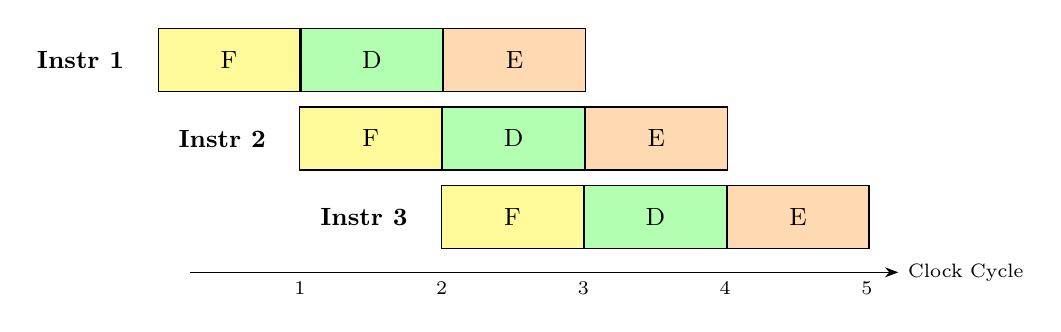
\begin{tikzpicture}[
    stage/.style={draw, rectangle, minimum width=1.8cm, minimum height=0.8cm, align=center, font=\small},
    arr/.style={-{Stealth}, thick}
  ]
  % Instruction 1
  \node[stage, fill=yellow!40] (f1) at (0,2) {F};
  \node[stage, fill=green!30, right=0pt of f1] (d1) {D};
  \node[stage, fill=orange!30, right=0pt of d1] (e1) {E};
  \node[left=0.3cm of f1, font=\small\bfseries] {Instr 1};

  % Instruction 2
  \node[stage, fill=yellow!40] (f2) at (1.8,1) {F};
  \node[stage, fill=green!30, right=0pt of f2] (d2) {D};
  \node[stage, fill=orange!30, right=0pt of d2] (e2) {E};
  \node[left=0.3cm of f2, font=\small\bfseries] {Instr 2};

  % Instruction 3
  \node[stage, fill=yellow!40] (f3) at (3.6,0) {F};
  \node[stage, fill=green!30, right=0pt of f3] (d3) {D};
  \node[stage, fill=orange!30, right=0pt of d3] (e3) {E};
  \node[left=0.3cm of f3, font=\small\bfseries] {Instr 3};

  % Clock cycle labels
  \foreach \x/\c in {0/1, 1.8/2, 3.6/3, 5.4/4, 7.2/5} {
    \node[below, font=\scriptsize] at (\x+0.9, -0.7) {\c};
  }
  \node[font=\scriptsize, right] at (8.5, -0.7) {Clock Cycle};
  \draw[-{Stealth}] (-0.5,-0.7) -- (8.5,-0.7);
\end{tikzpicture}%
}
\caption{Three-stage pipeline timing diagram: 3 instructions complete in 5 cycles.}
\label{fig:pipeline-3stage}
\end{figure}

Pipelining is possible because the Fetch, Decode, and Execute operations use \emph{independent resources}: Fetch uses the external buses, Decode uses the instruction decoder, and Execute uses the ALU. Since these units do not interfere with one another, they can operate concurrently on different instructions.

\begin{keyresult}[title={Key Result: Pipeline Speedup}]
  For an $k$-stage pipeline executing $n$ instructions, the total number of cycles is $k + (n - 1)$, compared with $k \cdot n$ for sequential execution. As $n$ grows large the pipeline approaches an ideal throughput of \textbf{one instruction per clock cycle}.
\end{keyresult}

\subsection{Pipeline Efficiency}
\label{sec:pipeline-efficiency}

The efficiency of a pipeline is maximised when the pipeline is \emph{fully filled}---that is, every stage is actively processing an instruction. Consider a 4-stage pipeline with stages Fetch (F), Decode (D), Execute (E), and Store (S). It takes 4 cycles to fill the pipeline and release the first instruction. After the pipeline is filled, however, one instruction completes every cycle, giving the effect of executing one instruction per clock cycle.

More complex application processors commonly employ 10 or more pipeline stages to further increase clock frequency, though deeper pipelines also increase the penalty when conflicts arise.

\section{Pipeline Conflicts}
\label{sec:pipeline-conflicts}

Pipeline conflicts (also called \emph{hazards}) are events that disrupt the smooth flow of instructions through the pipeline. They typically cause one of two outcomes: a temporary \emph{stall} (halt) of the pipeline, or a \emph{flush} in which partially processed instructions are discarded and the pipeline must be refilled. Both outcomes increase total execution time and reduce effective throughput.

Three sources of pipeline conflict are examined: resource conflicts, data dependency conflicts, and branch conflicts.

\subsection{Resource Conflict (Structural Hazard)}
\label{sec:resource-conflict}

\begin{definition}[Resource Conflict]
\label{def:resource-conflict}
  A resource conflict occurs when two instructions in different pipeline stages attempt to access the \emph{same hardware resource} during the same clock cycle.
\end{definition}

\begin{example}[Memory Contention]
\label{ex:resource-conflict}
In a 4-stage pipeline (F--D--E--S), suppose Instruction~1 reaches the Store stage and needs to write a result back to memory in the same cycle that Instruction~4 enters the Fetch stage and needs to read an instruction from the same memory. Both cannot use the memory bus simultaneously, creating a resource conflict.
\end{example}

Resource conflicts are resolved by providing sufficient independent resources for each pipeline stage. Modern pipeline processors typically include multiple internal buses (data bus, instruction bus, peripheral bus), separate instruction and data caches (Harvard architecture), and dedicated control and processing units so that all stages can operate simultaneously without contention.

\begin{examtip}[title={Exam Tip: Resolving Resource Conflicts}]
  The key solution to resource conflicts is \textbf{resource duplication}---for instance, using separate instruction memory and data memory (or caches) so that Fetch and Store can access memory simultaneously without conflict.
\end{examtip}

\subsection{Data Dependency Conflict (Data Hazard)}
\label{sec:data-dependency}

\begin{definition}[Data Dependency Conflict]
\label{def:data-dependency}
  A data dependency conflict arises when the source operand of the current instruction is the destination operand of a prior instruction that has not yet completed its Store stage. The current instruction reads a stale (old) value instead of the updated one.
\end{definition}

This is not an issue in a sequential CPU because each instruction fully completes before the next begins, so registers always hold up-to-date values. In a pipeline, however, the overlapping execution means a dependent instruction may reach its Execute stage before the prior instruction has stored its result.

\begin{example}[Data Dependency in a 4-Stage Pipeline]
\label{ex:data-dependency}
Consider the following code with initial register values $R1 = \texttt{0x2}$, $R2 = \texttt{0x0}$, $R3 = \texttt{0x5}$:
\begin{lstlisting}
ADD R2, R2, R1   ; R2 = R2 + R1 = 0x0 + 0x2 = 0x2
SUB R3, R3, R2   ; R3 = R3 - R2 (should use R2 = 0x2)
\end{lstlisting}
In a 4-stage pipeline (F--D--E--S), when \texttt{SUB} reaches the Execute stage (cycle~4), \texttt{ADD} is simultaneously in the Store stage. The updated value of $R2$ (\texttt{0x2}) has not yet been written back, so \texttt{SUB} reads the old value $R2 = \texttt{0x0}$ and computes $R3 = \texttt{0x5} - \texttt{0x0} = \texttt{0x5}$ instead of the correct $R3 = \texttt{0x5} - \texttt{0x2} = \texttt{0x3}$.
\end{example}

The exact number of instructions that must separate a producer and consumer to avoid a data hazard depends on the pipeline depth and design.

\subsubsection{Resolution: Stalling the Pipeline}
\label{sec:stall}

Hardware circuitry can detect data dependencies by comparing the destination register identifier in the Execute stage with the source register identifier(s) in the Decode stage. When a match is found, the dependent instruction is \emph{stalled} at the Decode stage until the prior instruction completes and the correct value is available. In the example above, stalling the \texttt{SUB} instruction for one cycle allows \texttt{ADD} to finish its Store stage, after which \texttt{SUB} reads $R2 = \texttt{0x2}$ and correctly computes $R3 = \texttt{0x3}$.

\subsubsection{Resolution: Inserting NOP Instructions}
\label{sec:nop}

Alternatively, the \emph{compiler} can detect data dependencies during compilation and insert explicit \texttt{NOP} (No Operation) instructions between dependent instructions. The \texttt{NOP} occupies a pipeline slot without performing any useful work, effectively delaying the dependent instruction by one cycle so that the updated value is available by the time it reaches the Execute stage. This approach yields the correct result but increases total execution time because an extra instruction must pass through the pipeline.

\begin{warning}[title={Warning: Stall vs.\ NOP}]
  Stalling is a \emph{hardware} mechanism---the pipeline control logic detects the hazard at run time and pauses the dependent stage. NOP insertion is a \emph{software/compiler} mechanism---the compiler inserts dummy instructions at compile time. Both introduce a one-cycle delay (for a 4-stage FDES pipeline with adjacent dependent instructions), but NOPs increase the total instruction count in the program.
\end{warning}

\section{Branch Conflicts (Control Hazards)}
\label{sec:branch-conflict}

\subsection{Branch Instruction Behaviour}
\label{sec:branch-behaviour}

A branch instruction (e.g.\ \texttt{BEQ}, \texttt{BNE}) performs two operations that both require computation: evaluating the branch condition (e.g.\ checking the Zero flag) and calculating the branch target address using the ALU. These operations naturally occur during the Execute (E) stage of the pipeline.

The problem is that while the branch instruction is being decoded and executed, the processor has already fetched one or more subsequent instructions into the pipeline. If the branch is \emph{taken}, these instructions are incorrect and must be discarded (\emph{flushed}). The number of cycles wasted by this flushing is called the \textbf{branch delay}, and the pipeline slots occupied by the discarded instructions are called \textbf{delay slots}.

\begin{definition}[Branch Delay]
\label{def:branch-delay}
  The branch delay is the number of clock cycles wasted when the pipeline must be flushed due to a taken branch. It equals the number of pipeline stages between the Fetch of the instruction after the branch and the stage at which the branch decision is resolved.
\end{definition}

\begin{example}[Two-Cycle Branch Delay]
\label{ex:branch-delay}
In a 4-stage pipeline where the branch decision is made in the Execute stage, by the time the branch target is known, two subsequent instructions (I and J) have already been fetched and partially processed. If the branch is taken, both must be discarded, resulting in a 2-cycle branch delay.
\end{example}

\subsection{Reducing Branch Delay}
\label{sec:reduce-branch-delay}

Branch delay can be reduced by moving the branch decision \emph{earlier} in the pipeline. By introducing an additional adder in the Decode stage to compute the branch target address and resolving the branch condition at the Decode stage instead of Execute, the branch outcome is known one stage earlier. In this configuration, only one instruction (the one fetched immediately after the branch) needs to be discarded if the branch is taken, reducing the branch delay to \textbf{one cycle}.

\subsection{Delayed Branching}
\label{sec:delayed-branching}

\begin{definition}[Delayed Branching]
\label{def:delayed-branching}
  Delayed branching is a pipeline strategy in which the processor \emph{always executes} the delay slot instruction(s) immediately following a branch, regardless of whether the branch is taken or not. No instructions are ever discarded, eliminating wasted cycles.
\end{definition}

Delayed branching can be viewed as a configurable feature of the processor:

\paragraph{Delayed branching disabled.} When the branch is taken, the delay slot instructions are discarded to preserve program correctness, at the cost of wasted cycles (branch delay).

\paragraph{Delayed branching enabled.} The delay slot instructions are always executed. However, if the original delay slot instructions (I and J) would produce incorrect results when the branch is taken, the programmer or compiler must \textbf{rewrite the code} to fill the delay slots with \emph{independent instructions} instead.

\subsubsection{Requirements for Delay Slot Instructions}
\label{sec:delay-slot-requirements}

The instructions placed in delay slots must satisfy several conditions:

\begin{enumerate}
  \item \textbf{Independence from the branch decision.} They must not modify any register or flag that affects the branch condition. For example, if a \texttt{BEQ} instruction depends on the Zero flag, the delay slot instruction must not alter the Zero flag (recall that all instructions are assumed to update condition flags by default, i.e.\ ADD behaves as ADDS).
  \item \textbf{Always executed in the original program.} They must be instructions that would have been executed regardless of whether the branch is taken or not. This typically means they are instructions that appear \emph{before} the branch in the original program sequence.
  \item \textbf{Loop context.} If the branch is part of a loop, the delay slot instructions should be sourced from within the loop body, since they will execute on every iteration.
  \item \textbf{Fallback.} If no suitable independent instruction can be found, the delay slot must be filled with a \texttt{NOP} to preserve correctness.
\end{enumerate}

\begin{example}[Code Rewriting for Delayed Branching]
\label{ex:delayed-branching}
\leavevmode
\begin{lstlisting}
; Original code:         ; Rewritten code:
  Instr 1                  Instr 1
  Instr 2                  BEQ Next
  Instr 3                  Instr 2    ; delay slot 1
  BEQ Next                 Instr 3    ; delay slot 2
  Instr I                  Instr I
  Instr J                  Instr J
  Next: Instr K            Next: Instr K
\end{lstlisting}
If Instructions~2 and~3 are independent of the branch decision, they can be moved \emph{after} the \texttt{BEQ} instruction to fill the delay slots. The processor executes them during the branch delay period, achieving zero wasted cycles.
\end{example}

\begin{keyresult}[title={Key Result: Delayed Branching}]
  When delayed branching is enabled and the delay slots are filled with independent instructions, the branch delay is effectively \textbf{zero}---no cycles are wasted. If independent instructions cannot be found, NOPs must fill the delay slots, and the performance benefit is lost.
\end{keyresult}

\subsection{Dynamic Branch Prediction}
\label{sec:branch-prediction}

\begin{definition}[Dynamic Branch Prediction]
\label{def:branch-prediction}
  Dynamic branch prediction uses hardware circuitry to \emph{guess} the outcome of a conditional branch before it is resolved. A \textbf{branch history table} stores the predicted target address and the predicted outcome (taken/not taken) for each branch instruction encountered.
\end{definition}

The prediction mechanism works as follows:

\begin{enumerate}
  \item When a branch instruction is fetched, the processor looks up the branch history table using the branch instruction's address.
  \item If an entry exists, the processor speculatively fetches instructions from the predicted target address.
  \item When the branch is resolved during the Execute (or Decode) stage:
    \begin{itemize}
      \item If the prediction was \textbf{correct}, execution continues normally with no wasted cycles.
      \item If the prediction was \textbf{incorrect}, the speculatively fetched instructions are flushed (wasting cycles), and the prediction bit and target address in the table are updated for future reference.
    \end{itemize}
\end{enumerate}

\begin{examtip}[title={Exam Tip: Branch Prediction vs.\ Delayed Branching}]
  Branch prediction and delayed branching are two distinct strategies for mitigating branch delay. Prediction is a \emph{hardware} approach that guesses the branch outcome, while delayed branching is a \emph{software/architectural} approach that restructures the code so delay slot instructions are always useful. Both can reduce or eliminate branch delay, but prediction incurs a penalty when the guess is wrong, whereas delayed branching requires finding suitable independent instructions.
\end{examtip}

\section{Note on ARM Instructions in Pipeline Examples}
\label{sec:arm-pipeline-note}

The pipeline examples in this module use ARM assembly instructions for illustration, but with the following simplifying assumptions:

\begin{itemize}
  \item The pipeline structure discussed is \textbf{not} the actual ARM Cortex pipeline.
  \item All ARM instructions are assumed to occupy exactly \textbf{one word} and each pipeline stage takes exactly \textbf{one clock cycle}.
  \item The `S' suffix is enabled by default on all instructions---i.e.\ every instruction updates the condition flags (e.g.\ \texttt{ADD} behaves as \texttt{ADDS}, \texttt{MOV} as \texttt{MOVS}).
\end{itemize}

\section{Real-World Connection: ARM Cortex-M3/M4}
\label{sec:arm-cortex}

The ARM Cortex-M3 and M4 processors use a \textbf{3-stage pipeline} (Fetch, Decode, Execute) with a branch speculation mechanism. When a branch instruction reaches the Decode stage, the processor speculatively fetches the branch destination instruction in parallel. During the Execute stage, the branch is resolved:

\begin{itemize}
  \item If the branch is \emph{not taken}, the next sequential instruction is already available.
  \item If the branch is \emph{taken}, the branch target instruction has been pre-fetched during the Decode stage and is available immediately when the decision is made.
\end{itemize}

This speculation mechanism reduces branch delay to near zero in many cases, illustrating how real-world processors combine pipeline design with predictive hardware to maintain high throughput.

\end{document}
